\chapter{Reelle Rekonstruktion}
\label{sec:real} 

Der entwickelte Szenenrekonstrukionsalgorithmus wird im Folgenden anhand eines realen Stereoaufbaus getestet. Anders als bei den synthetischen Bilddaten im Beispiel zuvor, muss beim arbeiten mit reellen Stereobildern mit einer Fehleranfälligkeit der Bilddaten gerechnet werden. Liegt beispielsweise bei der Bestimmung von korrespondierenden Punkten eine Ecke zwischen zwei Pixel, so kann optisches Rauschen, welches in realen Aufnahmen präsent ist, dazu führen dass die Ecke in gleichen Bildern an verschiedenen Pixel erkannt wird. Diese Abweichung der Punktekorrespondenz führt dazu, dass die in Kapitel \ref{sec:EpiolarContraints} definierten epipolaren Bedingungen nicht zur Gänze mehr erfüllt werden. In diesem Kapitel wird Hauptsächlich darauf eingegangen, welche Auswirkungen diese Ungenauigkeiten auf die Bestimmung der Fundamentalmatrix, der essentiellen Matrix, der extrinsischen Kameraparameter und der anschließenden Rekonstruktion der Szene durch Triangulierng haben und wie man ihnen entgegenwirken kann. In Abbildung \ref{fig:ArbeitsProzessReell}, ist der Arbeitsprozess für den reellen Fall zu sehen. Der Ablauf im Allgemeinen bleibt beständig.

%Hierzu wurde der Ursprüngliche Algorithmus um bestimmte Funktionen erweitert, welche im Verlauf des Kapitels genau erläutert werden. Abbildung \ref{fig:ArbeitsProzessReell} zeigt den Ablauf für die Reelle Rekonstruktion. \\
%
%Bildfehler genauer beschreiben und lösungsansatz skizzieren

\begin{figure}[!htb]
	\centering
	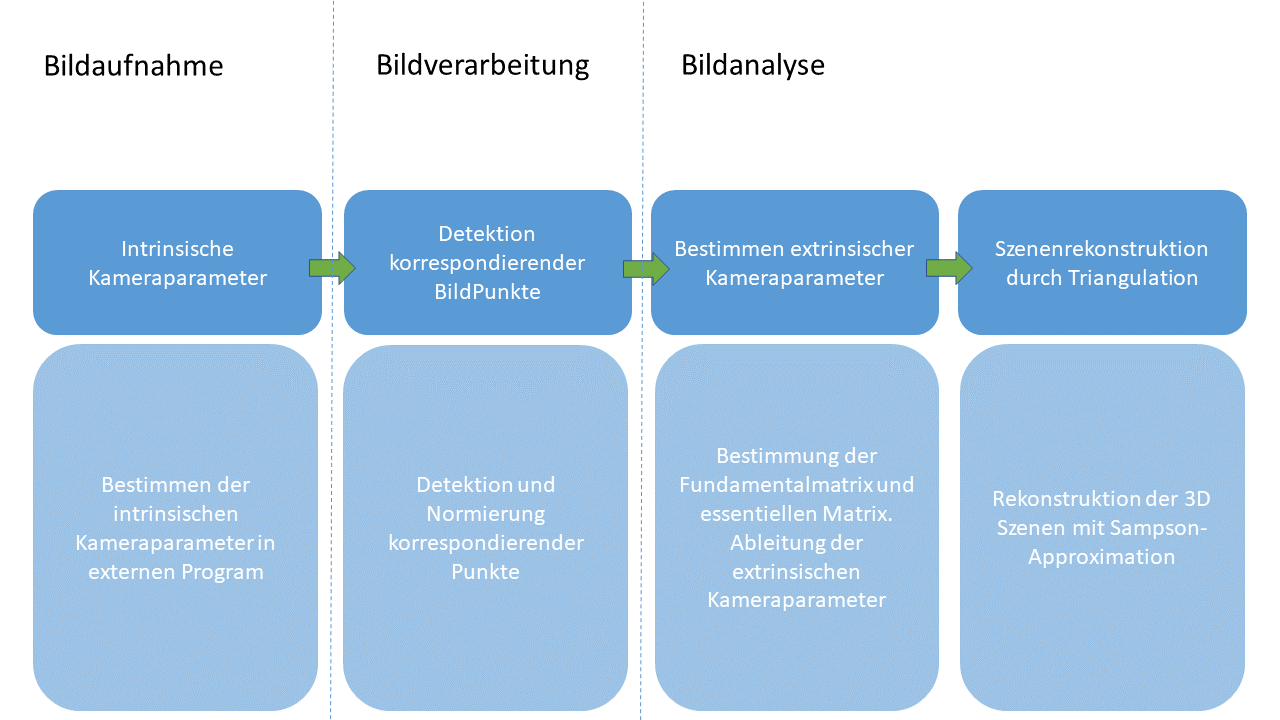
\includegraphics[width=1.\linewidth]{images/NEU_real_Arbeitsprozess.png}
	\caption[Ablaufdiagramm für die reelle Rekonstruktion]{Ablaufdiagramm für die reelle Rekonstruktion}
	\label{fig:ArbeitsProzessReell}
\end{figure}

%\begin{minipage}{\linewidth}
%	\centering
%	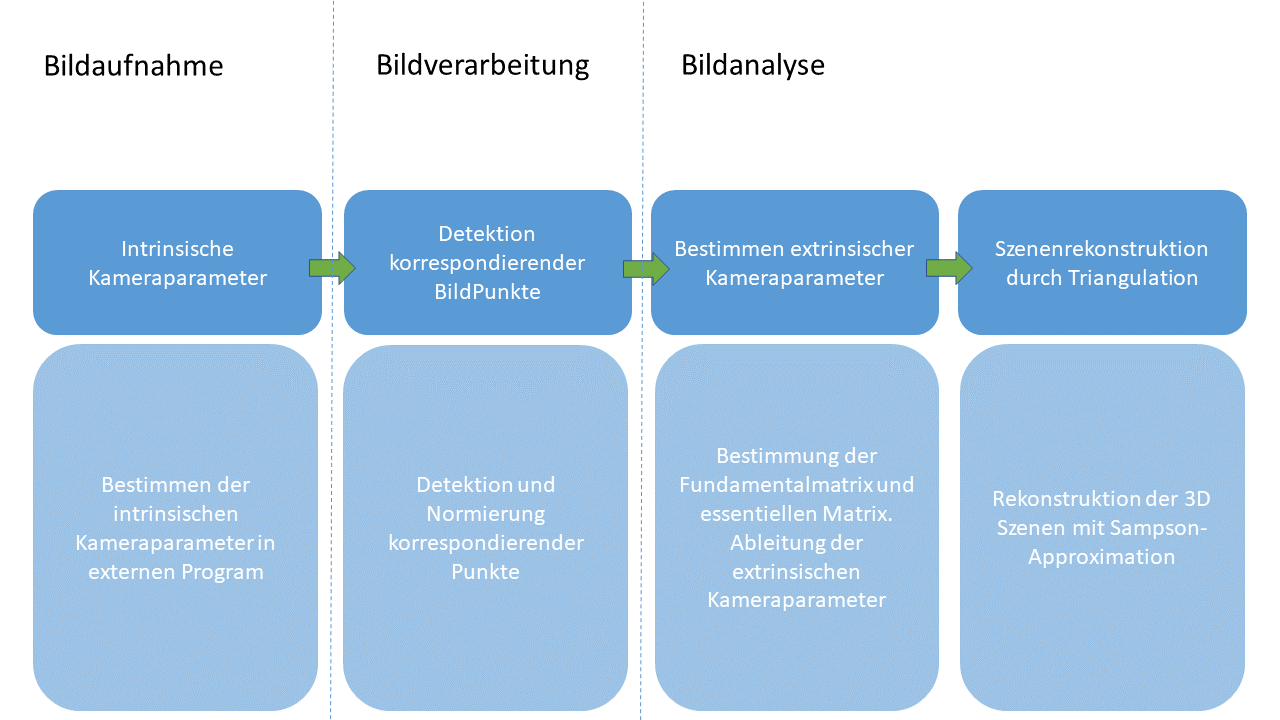
\includegraphics[width=1.\linewidth]{images/NEU_real_Arbeitsprozess.png}
%	\captionof{figure}{Ablaufdiagramm für die reelle Rekonstruktion}
%	\label{fig:ArbeitsProzessReell}
%\end{minipage}\\ \\

Zu Beginn wird der Stereoaufbau vorgestellt. Danach folgt die Korrespondenzanalyse, in welcher zwei Möglichkeiten aufgeführt werden, wie Punktekorrespondenzen aus den Stereoaufnahmen gewonnen werden können. Der Normierte-Acht-Punkt-Algorithmus, stellt eine für reale Bilddaten leicht veränderte Fassung des bereits bekannten Acht-Punkt-Algorithmus vor. Mit dessen Hilfe ist es möglich die Auswirkungen der Abweichungen in den Punktekorrespondenzen auf ein Minimum zu reduzieren. Nach der Bestimmung der Fundamentalmatrix durch den Normierten-Acht-Punkt-Algorithmus, wird diese auf ihre Gültigkeit kontrolliert. Hierzu werden vor allem die Singulärwerte der Fundamentalmatrix genauer betrachtet und welche Auswirkungen sie auf die Epipolargeometrie haben. Als nächstes wird die aus der Fundamentalmatrix bestimmte essentielle Matrix überprüft. Auch hier wird auf die Eigenschaften der Singulärwerte der essentiellen Matrix eingegangen.
\pagebreak

Danach wird eine Triangulierungsmethode nach \textit{Hartley \& Zisserman} \cite{HZ} vorgestellt, die über ein Näherungsverfahren eine Triangulation zwischen ungenauen korrespondierenden Punkten ermöglicht. Der letzte Abschnitt des Kapitels befasst sich dann mit der reellen Rekonstruktion bei unterschiedlichen Kameraauflösungen. \\



%Zunächst wird der Stereoskopische Aufbau kurz erläutert. 
%
%Der selbe Arbeitsprozess soll nun auch auf ein Realbeispiel mit Bildern zweier Kameras durchgeführt werden.
%
%Für die Kalibrierung der intrinsischen Kameraparameter wird auf ein externes Programm zurückgegriffen.
%
%Der Arbeitsprozess wird ähnlich dem des Minimalbeispiels ablaufen\\
%
%Auf bestimmte besonderheiten wird eingegangen, da reele Daten Fehleranfällig sind, genau so wie die detektion der korrespondierenden Bildpunkte
%
%
%Für die Stereoaufnahmen wurden die halbformat Kamera Canon 60 D und die Vollformatkamera 6D verwendet. Die Bilder wurden zunächst mit beiden Kameras bei selber Auflösung. Später wurden auch noch aufnahmen mit unterschiedlichen Auflösungen gemacht und ebenfalls die Stereoanalyse auf die Bildpaare angewandt.  \\


\section{Stereoaufbau}


Für die Stereobildaufnahme wurde eine Szene vor zwei nebeneinander platzierten Kameras aufgebaut. Beide Kameras wurden auf die Szene gerichtet. Abbildung \ref{fig:StereoaufbauReal} zeigt den entstandenen Stereoaufbau.\\

%Die räumliche Orientierung und Position von $C'$ wird also relativ zu $C$ berechnet und auch die Szene wird davon ausgehend, dass $C$ als Projektionsmatrix $P=[I|0]$ besitzt.

% dass sie leicht zueinander hin gedreht waren. Da die Canon 60D eine halbformatkamera ist, wurde sie weiter hinten als die Canon 6D positioniert. Somit konnte ungefähr der selbe Bildausschnitt der Szene mit beiden Kameras aufgenommen werden.\\



\begin{figure}[!htb]
	\centering
	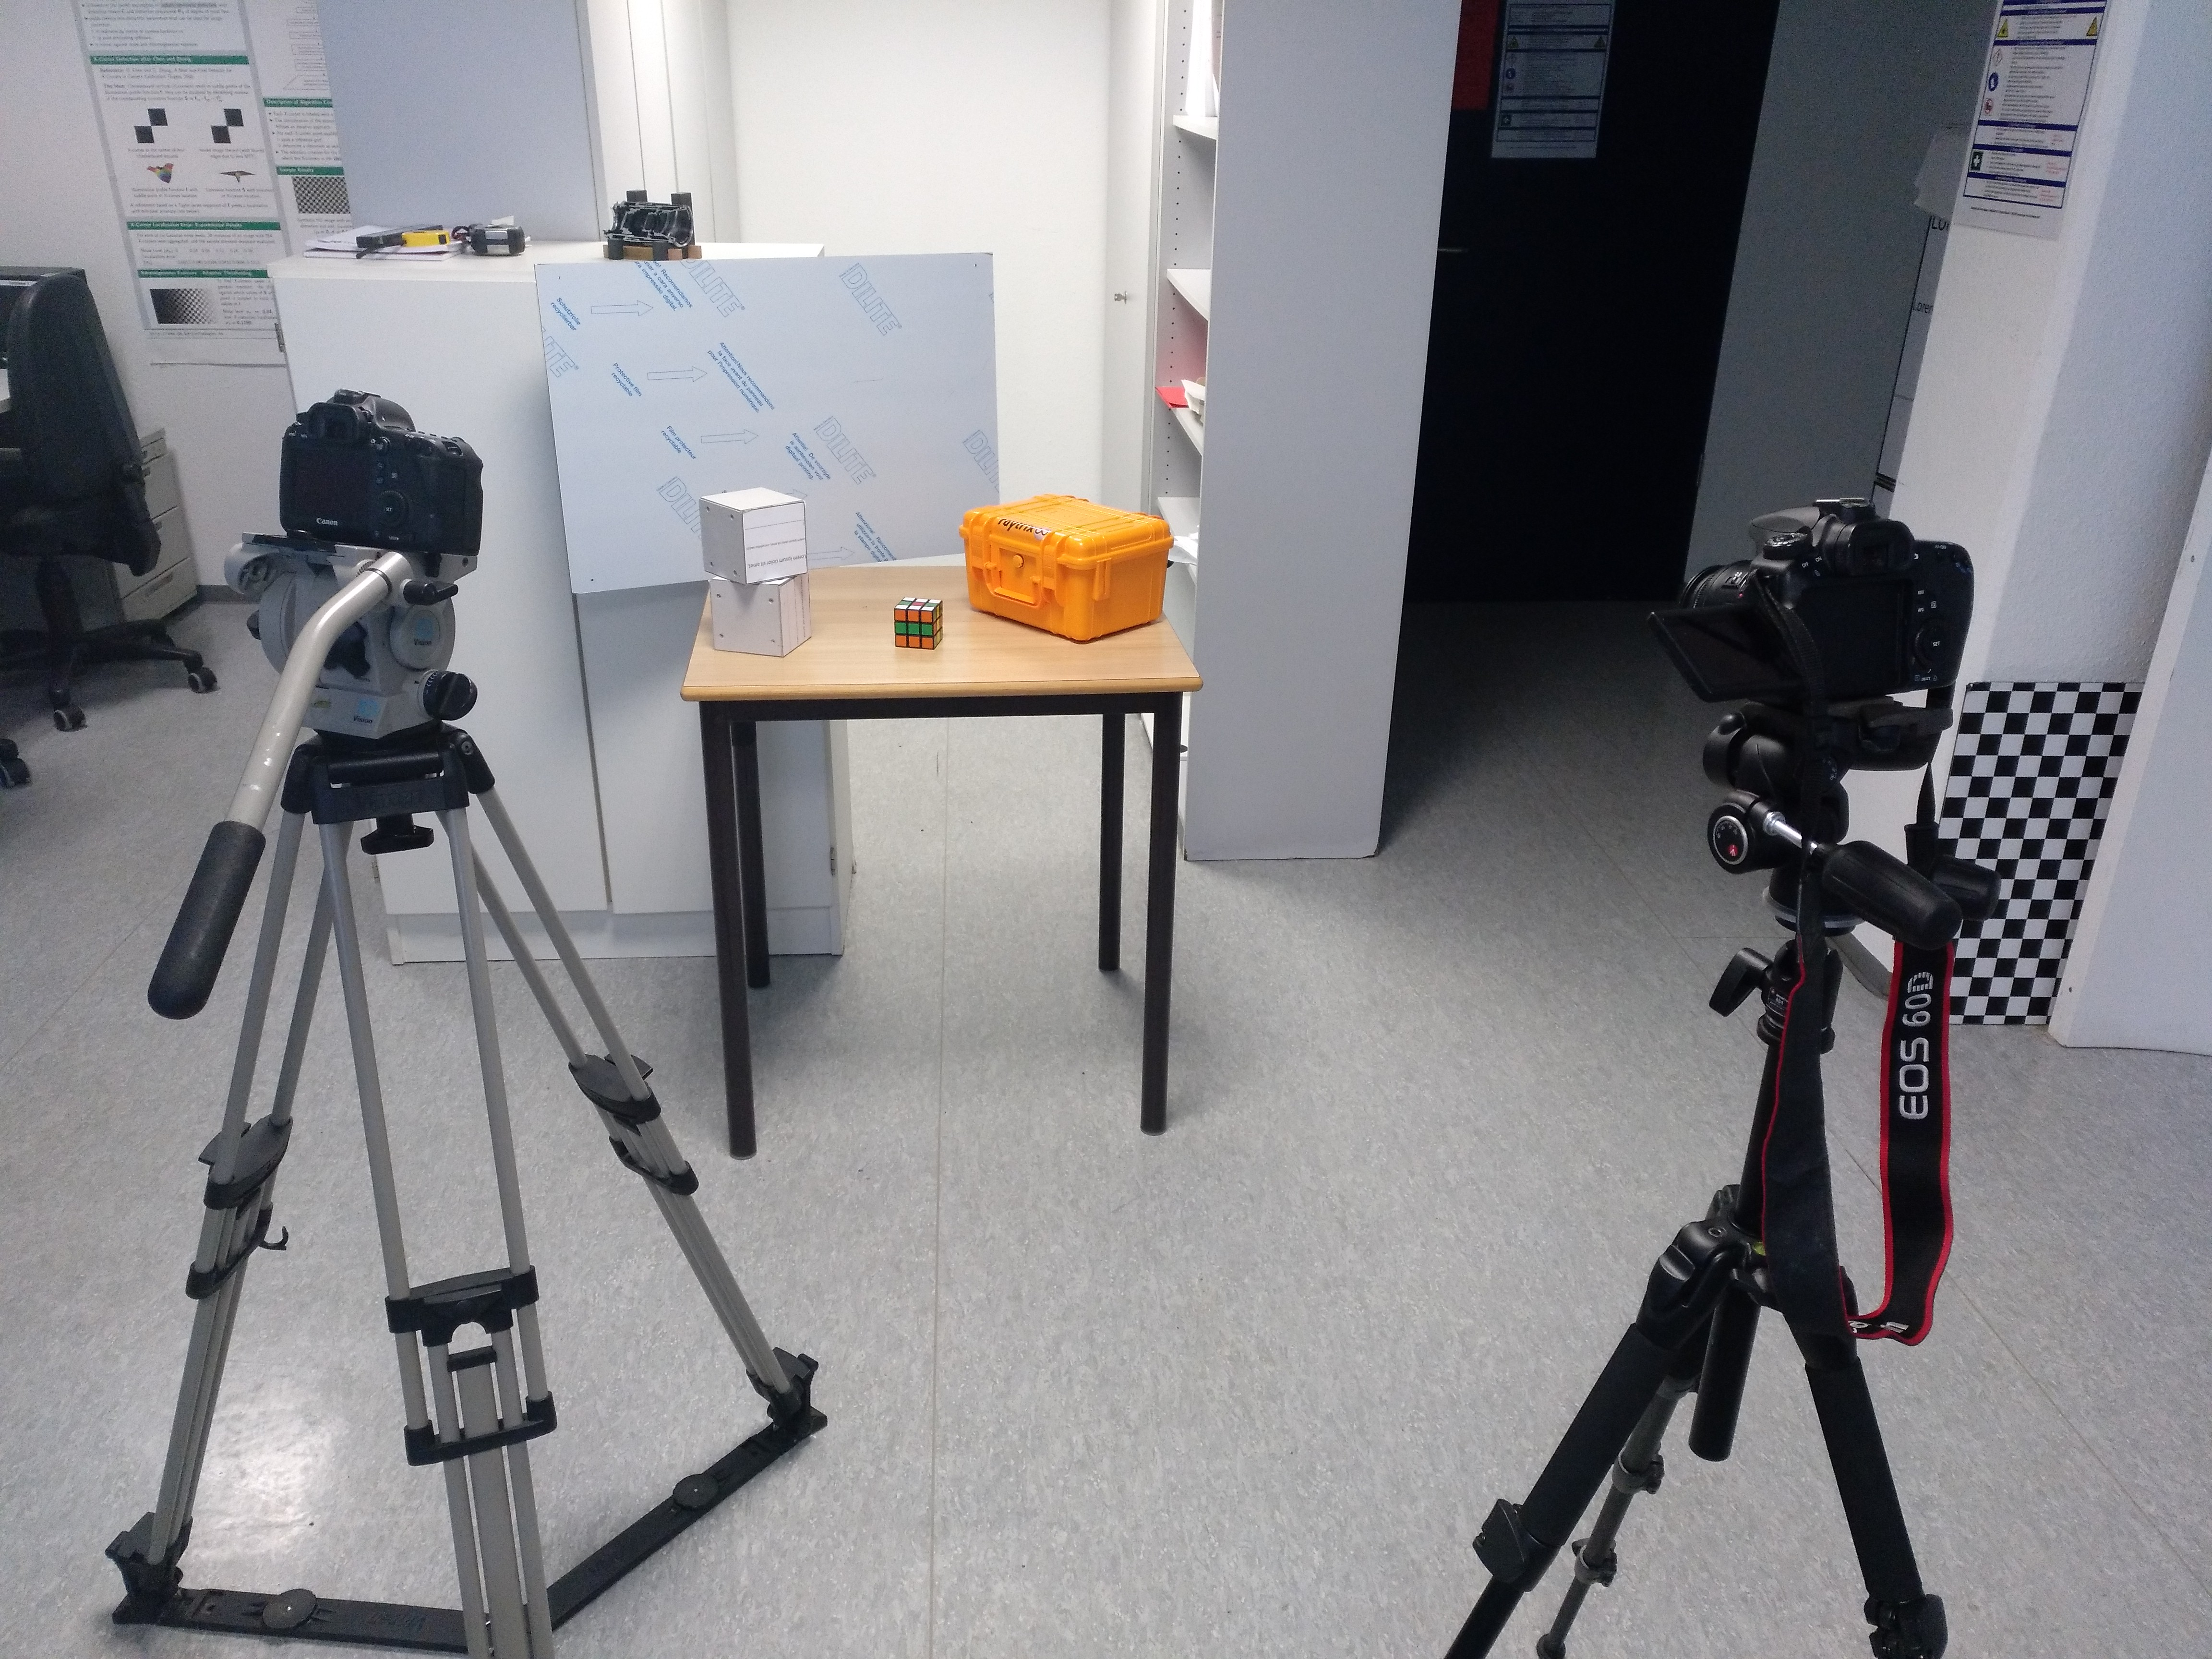
\includegraphics[width=.7\linewidth]{images/SetUpSameResolution.jpg}
	\caption[Stereoaufbau im Überblick]{Kamera eins $C$ befindet sich auf dem Bild links, Kamera zwei $C'$ befindet sich rechts im Bild. Auf dem Tisch zwischen den Kameras ist die in den Abbildungen \ref{fig:SurfLinks} und \ref{fig:SurfRechts} abgebildete Szene zu sehen. Beide Kameras sind auf die Szene gerichtet.}
	\label{fig:StereoaufbauReal}
\end{figure}


%\begin{minipage}{\linewidth}
%	\centering
%	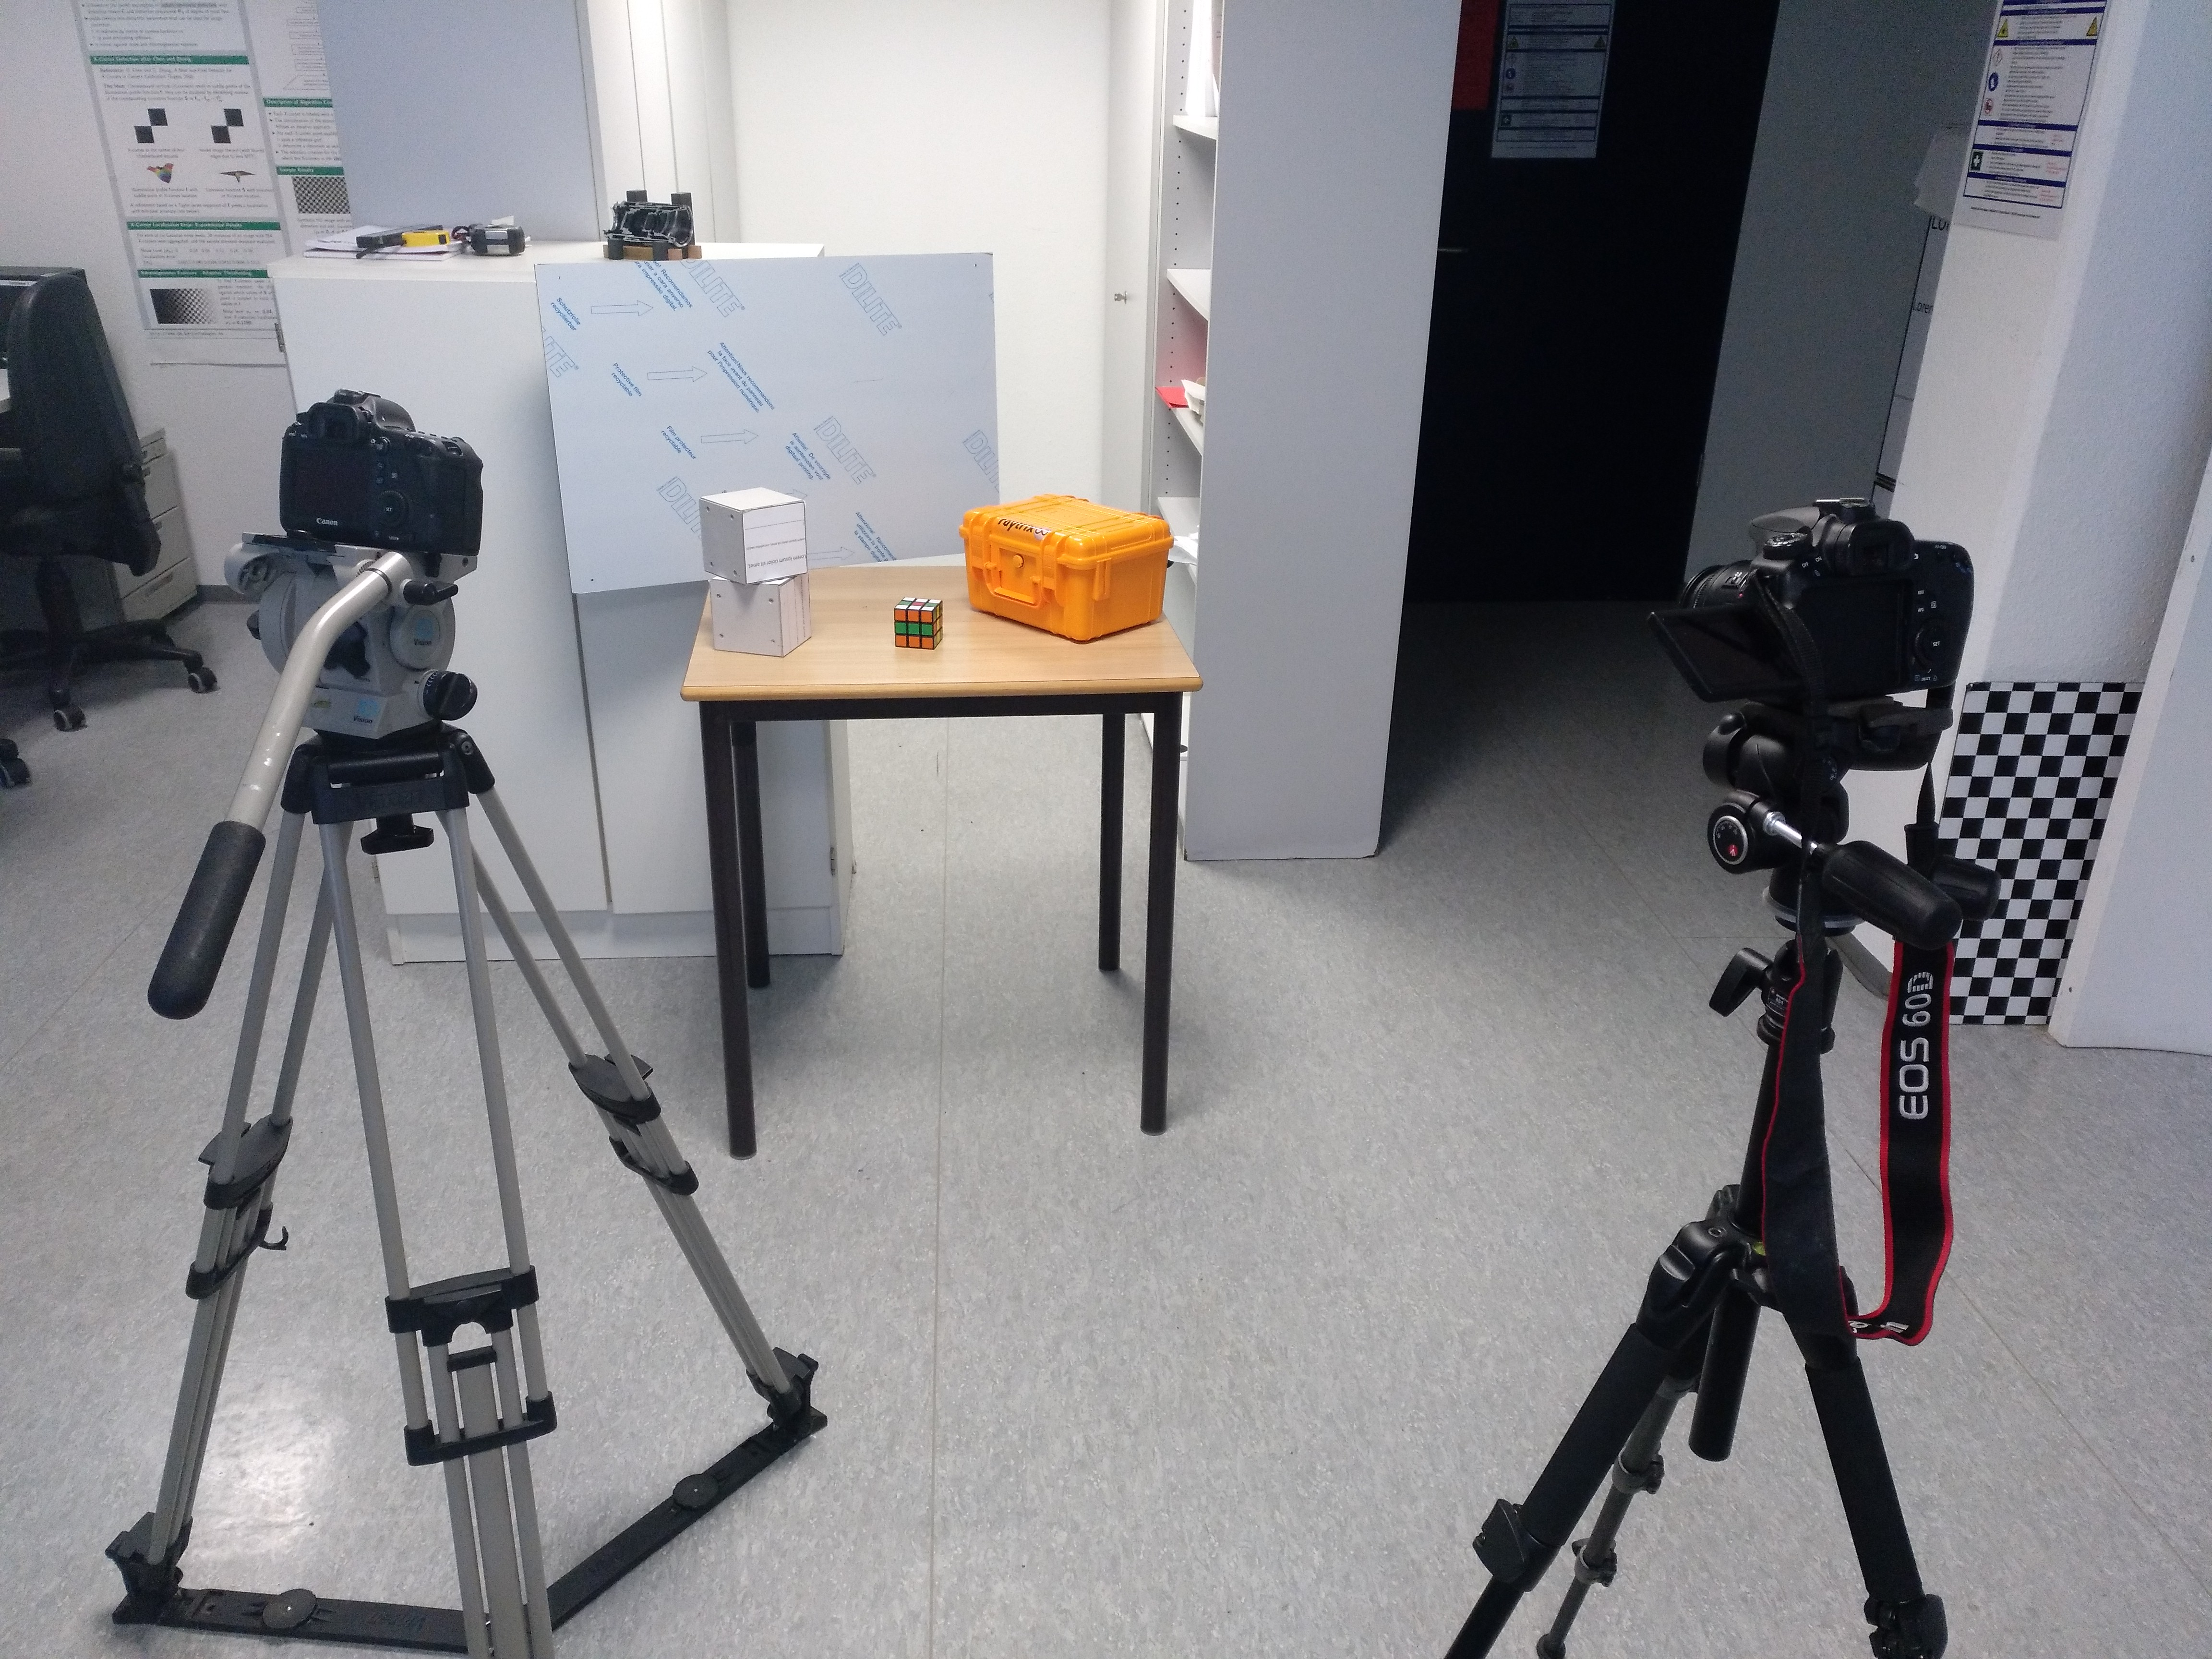
\includegraphics[width=.7\linewidth]{images/SetUpSameResolution.jpg}
%	\captionof{figure}{Szenenaufbau: Die Canon 60D befindet sich in dieser Abbildung auf der linken Seite, die Canon 60 D auf der rechten. Auf dem Tisch zwischen den Kameras ist die in den Abbildungen 6.1 und 6.1 abgebildete Szene zu sehen. Beide Kameras sind zu Szene hin gedreht.}
%	\label{fig:StereoaufbauReal}
%\end{minipage}\\

Die auf Abbildung \ref{fig:StereoaufbauReal} zu sehende linke Kamera wurde als primäre Kamera definiert. Die extrinsischen Kameraparameter für $C'$, werden dahingehend realiv zu $C$ bestimmt werden. Das Kamerakoordinatensystem $(C,\beta)$ entspricht somit gleich dem Weltkoordinatensystem $(O,\delta)$. Kamera zwei mit $(C',\beta')$ befindet sich auf der Abbildung rechts. Für beide Kameras wurden in einem externen Programm die intrinsischen Kameraparameter $K$ und $K'$ bestimmt. An den Stereoaufnahmen der Szene wird dann eine Korrespondenzanalyse durchgeführt.   

\section{Korrespondenzanalyse}


Für die Detektion von Punktekorrespondenzen bei Stereoaufnahmen einer dreidimensionalen Szene wurde eine bereits existierende Funktion von Mathematica genutzt\cite{Mathematica}. Die Funktion basiert auf dem Prinzip eines SURF-Algorithmus. SURF ist die Kurzform für \textit{Speeded Up Robust Features} und ist ein Rotations- und Skaleninvarianter Punkte Detektor und Deskriptor\cite{SURF,SIFTSURF}. Es werden Punkte an markanten Stellen in beiden Bildern detektiert, wie beispielsweise Eckpunkte oder Kanten. Die Umgebung eines jeden gefundenen Punktes wird durch einen Merkmalsvektor, dem Deskriptor, beschrieben. Die Deskriptoren beider Bilder werden abgeglichen und gleiche Punkte werden als korrespondierende Punkte gekennzeichnet\cite{SURF,SIFTSURF}. Die Abbildungen \ref{fig:SurfLinks} und \ref{fig:SurfRechts} zeigen die Ergebnisse nach der Anwendung des SURF-Algorithmus auf das Stereobildpaar. 
\pagebreak

Eine eigens implementierte alternative für die Korrespondenzanalyse zwischen Stereoaufnahmen eines zweidimensionalen Schachbretts wird in Kapitel \ref{sec:schachbrettAlg} vorgestellt.  


%	\minipage{0.48\textwidth}
%	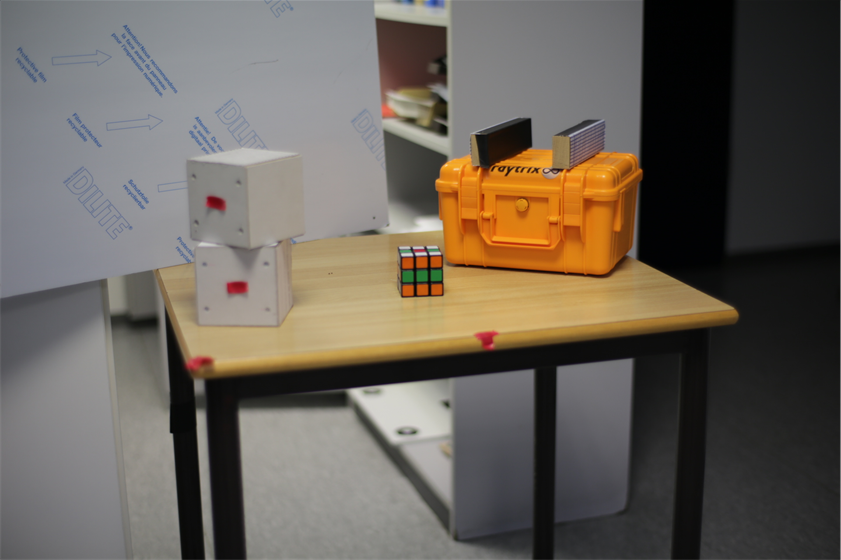
\includegraphics[width=\linewidth]{images/Points3DSceneLeft.png}
%	\caption{Aufnahme der Canon 6D von links}
%	\label{fig:awesome_image1}
%	\endminipage\hfill
%	\minipage{0.48\textwidth}
%	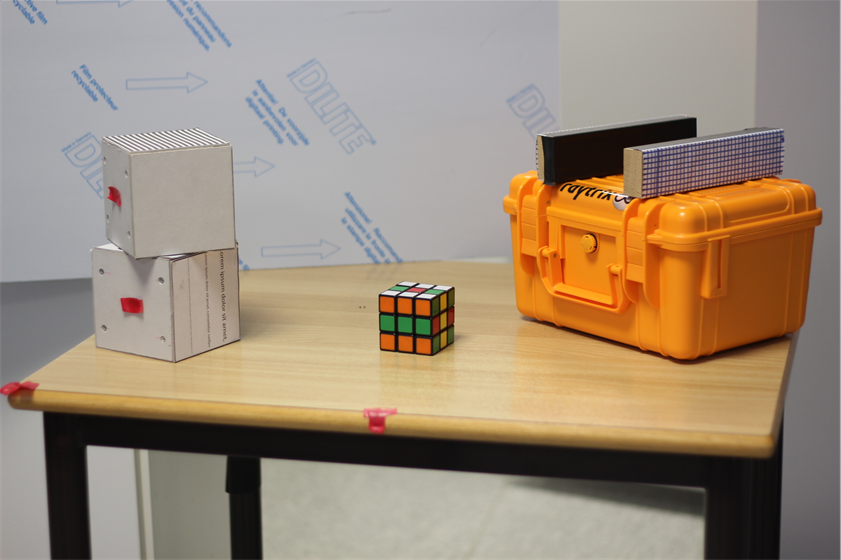
\includegraphics[width=\linewidth]{images/Points3DSceneRight.png}
%	\caption{Aufnahme der Canon 60D von rechts}
%	\label{fig:awesome_image2}
%	\endminipage\hfill
%\end{figure}
\begin{figure}[!htb]
	\minipage{0.48\textwidth}
	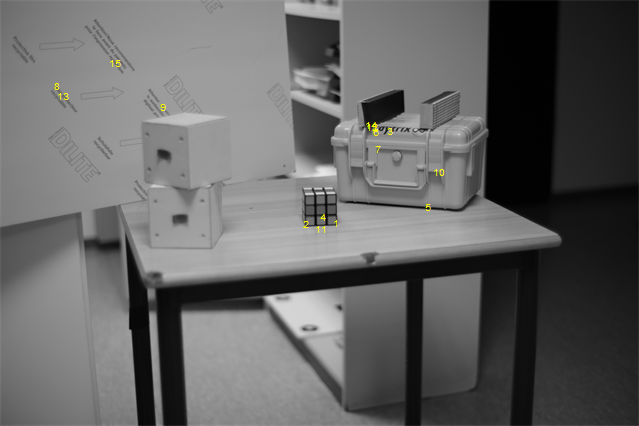
\includegraphics[width=\linewidth]{images/PointsDetectedLeft.png}
	\caption[Aufnahme von Kamera $C$]{Aufnahme von Kamera $C$}
	\label{fig:SurfRechts}
	\endminipage\hfill
	\minipage{0.48\textwidth}
	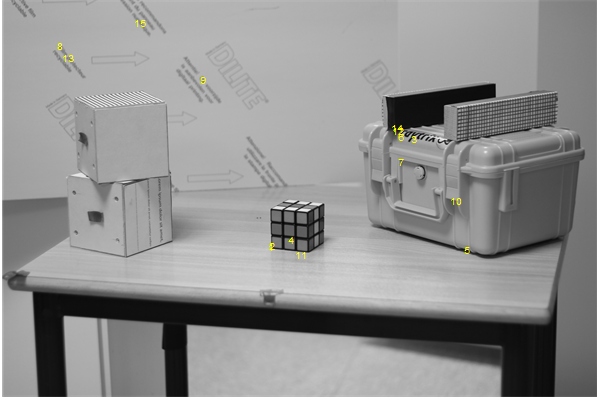
\includegraphics[width=\linewidth]{images/PointsDetectedRight.png}
	\caption[Aufnahme von Kamera $C'$]{Aufnahme von Kamera $C'$}
	\label{fig:SurfLinks}
	\endminipage\hfill
%	\caption{Die mit dem \textit{SURF}-Algorithmus gefundenen Punkte sind mit den gelben Ziffern im Bild gekennzeichnet. Abbildung a zeigt das Bild von $C$, die Abbildung b zeigt das Bild von $C'$}
\end{figure}
%\pagebreak

Die mit dem \textit{SURF}-Algorithmus gefundenen Punkte sind mit den gelben Ziffern in den Abbildungen \ref{fig:SurfLinks} und \ref{fig:SurfRechts} gekennzeichnet. Die Abbildung \ref{fig:SurfLinks} zeigt das Bild von $C$, die Abbildung \ref{fig:SurfRechts} zeigt das Bild von $C'$.\\

Die Detektion von Punktekorrespondenzen mit Detektionsalgorithmen, wie beispielsweise dem angewendeten SURF-Algorithmus, können immer Fehler und Abweichungen mit sich bringen. Die Ursprünge der Fehler können sowohl durch den Algorithmus als auch durch Fehler, wie Bildrauschen, in den Aufnahmen selbst entstehen. Diese Fehler wirken sich sowohl auf die Bestimmung der Abbildungsvorschriften $F$ und $E$ aus und somit auch auf die Genauigkeit der Szenenrekonstruktion\cite{HZ}. Im Folgenden werden sowohl die Fehler als auch Methoden für deren Minimierung vorgestellt.

\section{Normierter-Acht-Punkt-Algorithmus}

Trotz das der Acht-Punkt-Algorithmus eine einfache Methode zur Bestimmung der Fundamentalmatrix bietet, ist er sehr instabil sobald Fehler wie Ungenauigkeiten in Punktekorrespondenzen  auftreten\cite{HZ,Brooks}.\\

Die Ausmaße der Fehler lässt sich anhand der Kondition der Koeffizientenmatrix $A$ genauer feststellen. Als Kondition wird die Abhängigkeit der Lösung eines Problems von der Störung der Eingangsdaten beschrieben\cite{HZ8,ConditionNumber,Manocha}. Die Kondition lässt sich durch Bestimmung des kleinsten Eigenvektors der Matrixmultiplikation der Koeffizientenmatrix $A$ mit ihrer Transponierten $A^T$ herausfinden. Die Matrix $AA^T$ wird in die Matrizen $UDU^T$ zerlegt, wobei $U$ eine orthogonale und $D$ eine diagonale Matrix ist. Die Diagonaleinträge von $D$ sind in einer nicht ansteigenden Reihenfolge, woraus resultiert, dass der kleinste Singulärwert von $D$ mit der letzten Spalte von $U$ korrespondiert. Die letzte Spalte von $U$ is gleich dem kleinsten Eigenvektor von $AA^T$\cite{HZ8,ConditionNumber}. Wird angenommen, dass $AA^T$ eine 9 $\times$ 9- Matrix ist, so ergeben die Diagonaleinträge $d_1/d_9$ den Wert der Kondition. Je größer die Kondition ist, desto größer wirken sich schon kleinste Abweichungen der reinkommenden Bilddaten, auf die aus $A$ bestimmte Matrix $F$ aus. Erkenntlich wird eine schlechte Kondition dann zum Beispiel an einem Ungleichgewicht der Matrixeinträge von $F$\cite{HZ8}. Das bedeutet, dass sich die Matrixeinträge stark in ihren Größeneinheiten unterscheidet. \\

\begin{gather}
	F = \begin{pmatrix}
		10^{-8}&10^{-6}&10^{-4}\\
		10^{-7}&10^{-8}&10^{-3}\\
		10^{-4}&10^{-3}&10^{-2}\\
	\end{pmatrix}
\end{gather}.

Die epipolare Bedingung mit $m'^T_{\sigma'}Fm_\sigma = 0$ errechnet schon bei kleinste Abweichungen der Punktekorrespondenzen große Fehler. Die schlechte Kondition liegt laut $Hartley \& Zisserman$ an der weitflächigen Verteilung der homogenen Bildkoordinaten im Raum. Die heutigen Kameras können Bilder mit bis zu mehreren tausend Pixel aufnehmen. Ein Bildpunkt kann somit beispielsweise wie folgt aussehen.

\begin{gather}
	m_\sigma = \begin{pmatrix}
		1150\\2193\\1
	\end{pmatrix}
\end{gather}

$m_{\sigma\, x}$ und $m_{\sigma\, y}$ liegen in einem Bereich der sich um mehr als 1000 Pixel unterscheidet. Das bedeutet, dass sich die ersten beiden Koordinateneinträge um einen viel größeren Zahlenbereich befinden als ihre dritte Komponente. Um die Kondition möglichst klein zu halten, werden die Bildkoordinaten beider Bilder normiert\cite{HZ8,Brooks}. Normierte Koordinaten befinden sich in einem ausgeglicheneren Wertebereich und liegen nicht mehr weit verteilt im Raum\cite{HZ8}. Ihre Einträge entsprechen dem Folgenden Beispiel

 \begin{gather}
 	m_\sigma = \begin{pmatrix}
 		1.5\\1.193\\1
 	\end{pmatrix}
 \end{gather}.

Die Einträge der entstehende Fundamentalmatrix haben dann die Form

\begin{gather}
	F = \begin{pmatrix}
		10^{-3}&10^{-2}&10^{-2}\\
		10^{-2}&10^{-3}&10^{-2}\\
		10^{-2}&10^{-2}&10^{-2}\\
	\end{pmatrix}
\end{gather}.

Das hat zur Folge, dass die epipolare Bedingung  weniger stark auf ungenaue Punktekorrespondenzen reagiert. Die in Literaturquellen, vorgeschlagene Methode zur Normierung besteht darin den Schwerpunkt aller Punkte in den Ursprung des Sensorkoordinatensystems zu verschieben und die Bildpunkt so zu skalieren, dass ihr durchschnittlicher Abstand zum Ursprung $\sqrt{2}$ beträgt\cite{HZ,Ferid,Brooks}.\\


Für die Normierung wird pro Bild eine Transformationsmatrix $T$ und $T'$ definiert. Die Matrizen beinhalten sowohl eine Skalierung als auch eine Translation. Die Bestimmung der Matrix $T$ wird im Folgenden aufgezeigt. Zuerst wird der Schwerpunkt $s$ mit $s=\begin{pmatrix}
s_x\\
s_y
\end{pmatrix}$ der Punktemenge $p_n$ mit $p_n = \begin{pmatrix}
p_{nx}\\
p_{ny}
\end{pmatrix}$ berechnet, indem der Mittelwert aller Punkte $p_n$ berechnet wird.

\begin{gather}
	\begin{pmatrix}
		s_x\\
		s_y
	\end{pmatrix} = \frac{1}{n} \sum_{i = 1}^{n} \begin{pmatrix}
	p_ix\\
	p_iy
\end{pmatrix}
\end{gather}

Danach wird $s$ in den Ursprung verschoben. Die Punkte $x_n$ werden ebenfalls um den Wert von $s$ verschoben $x'_n = x_n - s$. Der Mittelwert aus den um $s$ verschobenen Punkten $x'_n$ ergibt den neuen Schwerpunkt $s_0$ im Koordinatenursprung. Als nächstes wird die Distanz jedes Punktes von $x'_n$ zu $s_0$ berechnet und der Mittelwert aller Distanzen, hier mit $d$ bezeichnet, berechnet. Die Matrix $T$ und $T'$ haben dann die folgende Form:

\begin{gather}
	T = \begin{pmatrix}
		\frac{\sqrt{2}}{d}&0&-s_x\\
		0&\frac{\sqrt{2}}{d}&-s_y\\
		0&0&1
	\end{pmatrix}\\
	T' = \begin{pmatrix}
	\frac{\sqrt{2}}{d'}&0&-s'_x\\
	0&\frac{\sqrt{2}}{d'}&-s'_y\\
	0&0&1
\end{pmatrix}
\end{gather}

Die originalen Bildpunkte des Stereobildpaares, werden mit den Matrizen $T$ und $T'$ verrechnet. Mit den Normierten Bildkoordinaten wird dann mit dem Acht-Punkte-Algorithmus eine Fundamentalmatrix $\hat{F}$ bestimmt\cite{HZ,HZ8,Ferid,Brooks}. Ist $\hat{F}$ aus den normierten Koordinaten bestimmt, wird sie mit $T$ und $T'$ wieder denormalisiert.

\begin{gather}
	F = T'^T\hat{F}T
\end{gather}



\subsection{Singularität der Fundamentalmatrix}
\label{sec:SingularityOfF}

Die aus den Punktekorrespondenzen bestimmte Fundamentalmatrix muss eine singuläre Matrix mit Rang 2 sein\cite{HZ,ZZGXr,Ferid}. Die Singularität der Fundamentalmatrix sorgt zum einen dafür das ihr rechter und linker Kern jeweils eine eindeutige Lösung für den Epipol des jeweiligen Bildes ergibt und die Epipolarlinien, welche mit $l = Fm_\sigma$ und $l' = F^Tm'_{\sigma'}$ berechnet werden, auch alle durch diese Epipole verlaufen\cite{HZ}. Durch Ungenauigkeiten in korrespondierenden Bildpunkten kann es dazu kommen, dass die aus dem Normierten-Acht-Punkt-Algorithmus bestimmte Fundamentalmatrix $\hat{F}$ in ihrem Rang steigt und somit keine singuläre Matrix mehr ist. Matrizen sind singulär, wenn sie keine Inverse besitzen, was durch as verschwinden der Determinante nachgewiesen werden kann\cite{FormelsammlungMatrizen}. Die Determinanten von $\hat{F}$ muss Null sein, damit sie eine singuläre Matrix ist.\\

Ist $\hat{F}$ durch den erhöhten Rang keine singuläre Matrix, so ergeben der linke und der rechte Kern von $\hat{F}$ keine eindeutigen Lösungen mehr für $e$ und $e'$ und die Epipolarlinien in beiden Bildern verlaufen dementsprechend auch nicht mehr durch genau einen Punkt, wie man in den Abbildungen \ref{fig:NoEpipoleWithF1} und \ref{fig:NoEpipoleWithF2} erkennen kann. Die Abbildungen bilden Epipolarlinien aus dem Stereobildpaar \ref{fig:SurfRechts} und \ref{fig:SurfLinks} ab. Die Ursache des erhöhten Ranges von $\hat{F}$ ist in ihren Singulärwerten von $F$ zu finden.\\

\pagebreak
%
%irgendwie sagen dass es durch verunreinigte daten zu fehlern im constraint kommt und die Fundamentalmatrix im Rang steigt.
%
%Die Fundamentalmatrix ist eine singuläre-Matrix und ist somit eine Matrix von Rang zwei. Di
%
%wird die Fundamentalmatrix durch eine Singulärwertszerlung von $A$ geschätzt, ist die Chance sehr hoch, dass das Ergebnis für $\hat{F}$ eine Matrix von Rang 3 ist. Sollte dies der Fall sein gehen die Epipolarlinien der Bilder nicht mehr durch genau einen Punkt, wie man in den Abbildungen 6.5 und 6.6 erkennen kann. Diese bilden Epipolarlinien in einem Stereobildpaar ab.\\

\begin{figure}[!htb]
	\minipage{0.48\textwidth}
	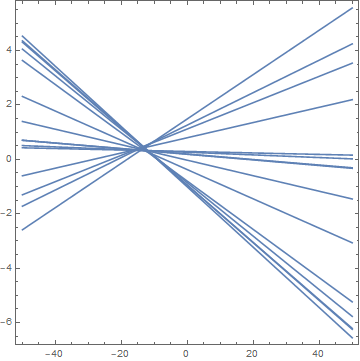
\includegraphics[width=\linewidth]{images/L_F_no_Constraint.png}
	\caption[Epipolarlinien $C$ ohne Singularität]{Epipolarlinien ohne \textit{Epipolar-constraint} im Bild der Canon 6D}
	\label{fig:NoEpipoleWithF1}
	\endminipage\hfill
	\minipage{0.48\textwidth}
	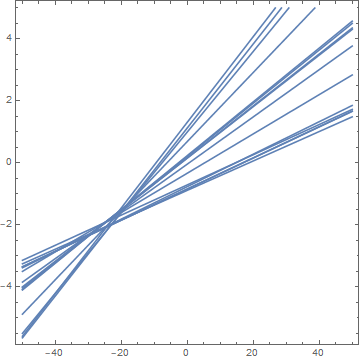
\includegraphics[width=\linewidth]{images/LPrime_PC2_F_no_Constraint.png}
	\caption[Epipolarlinien $C'$ ohne Singularität]{Epipolarlinien ohne \textit{Epipolar-constraint} im Bild der Canon 60D}
	\label{fig:NoEpipoleWithF2}
	\endminipage\hfill
	%	\caption{Die mit dem \textit{SURF}-Algorithmus gefundenen Punkte sind mit den gelben Ziffern im Bild gekennzeichnet}
\end{figure}

%Um eine gültige Fundamentalmatrix für den weiteren Arbeitsprozess zu generieren, kommt hier ein sogenannter \textit{singularity constraint} zum Einsatz.

Um mit dem Algorithmus weiter verfahren zu können, muss die Singularität in der noch normierten Fundamentalmatrix $\hat{F}$ erzwungen werden\cite{HZ}. Hierfür wird eine Singulärwertzerlegung an $\hat{F}$ durchgeführt, so dass $\hat{F}$ in $\hat{F} = U\Sigma V^T$ zerlegt wird. $\Sigma$ beinhaltet in einer Diagonalmatrix die Singulärwerte $D = \text{diag}(r,s,t)$. Die Diagonaleinträge erfüllen die Bedingung, dass $r \geq s \geq t $ gilt. Damit $\hat{F}$ zu einer singulären Matrix wird, muss für die Diagonaleinträge jedoch gelten, dass  $\Sigma = \text{diag}(r,s,0)$ ist. Diese Bedingung wird erzwungen, indem der letzte Eintrag $t$ auf $t = 0$ gesetzt wird. Die so modifizierte Fundamentalmatrix mit $\bar{F} = U\text{diag}(r,s,0)V^T$ wird dann wieder zusammengesetzt. Die Fundamentalmatrix $\bar{F}$ besitzt jetzt einen Rang 2 und ist singulär\cite{HZ}. $\bar{F}$ minimiert die Frobenius Norm $\parallel \hat{F} -\bar{F} \parallel$ und ist die nächste zum ursprünglichen $F$ liegende singuläre Matrix von Rang 2\cite{HZ,HZ8,FormelsammlungMatrizen}. \\

Werden aus $\bar{F}$ der rechte und linke Kern bestimmt, so ergeben sich eindeutige Lösungen für $e$ und $e'$ und die Epipolarlinien $l$ und $l'$ verlaufen jeweils durch ihre entsprechenden Epipole\cite{HZ}. Die Abbildungen \ref{fig:EpipoleWithF1} und \ref{fig:EpipoleWithF2} zeigen die Auswirkung der erzwungenen Singularität von $F$ auf dem Stereobildpaar \ref{fig:SurfRechts} und \ref{fig:SurfLinks}. Die Abbildungen \ref{fig:EpipoleWithF1Denorm} und \ref{fig:EpipoleWithF2Denorm} zeigen die selben Epipolarlinien nur ist $\bar{F}$ mit $T$ und $T'$ denormalisiert worden.\\



% Zu aller erst wird eine Singulärwertszerlegung an $F$ durchgeführt, so dass $\hat{F}$ in $\hat{F} = UDV^T$ zerlegt wird. $D$ beinhaltet in einer diagonalen Matrix die Singulärwerte $D = \text{diag}(r,s,t)$, welche die Bedingung $r \leq s \leq t $ erfüllen. 
% 
% Um nun den \textit{singularity-constraint} in $\hat{F}$ zu erzwingen, wird der letzte Singulärwert $t = 0$ gesetzt, so dass am Ende dasteht $D = \text{diag}(r,s,0)$. Danach werden die Matrizen $UDV^T$, wobei $D$ nun die modifizierten Singulärwerte beinhaltet, wieder zu $\hat{F}$ multipliziert. Die jetzt resultierende Fundamentalmatrix $\hat{F}$ besitzt den Rang 2. Der rechte und linke Kern ergeben wieder die Epipole und die Epipolarlinien verlaufen wieder durch eben diese Epipole. Die Abbildungen 6.7 und 6.8 zeigen die selben Epipolarlinien wie in 6.5 und 6.6 nachdem der \textit{singularity-constraint} in $\hat{F}$ erzwungen wurde. Die somit entstandene Matrix $\hat{F}$, ist die laut Frobenius norm, nächste zum ursprünglichen $\hat{F}$\cite{HZ}.

%Jetzt erst erfolgt die zuvor erwähnte denormierung von $\hat{F}$ durch $T$ und $T'$. Die Abbildungen 6.9 und 6.10 zeigen die Epipolarlinien im Originalbild mit denormierten Koordinaten.


\begin{figure}[!htb]
	\minipage{0.48\textwidth}
	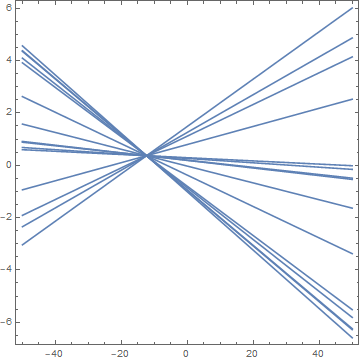
\includegraphics[width=\linewidth]{images/L_PC1_F_Constraint.png}
	\caption[Epipolarlinien in $C$ aus singulärer Fundamentalmatrix]{Die Abbildung zeigt, dass die Epipolarlinien auf der Aufnahme von $C$, nach dem Erzwingen der singularität in der normierten $\hat{F}$, alle durch den Epipol $e$ verlaufen}
	\label{fig:EpipoleWithF1}
	\endminipage\hfill
	\minipage{0.48\textwidth}
	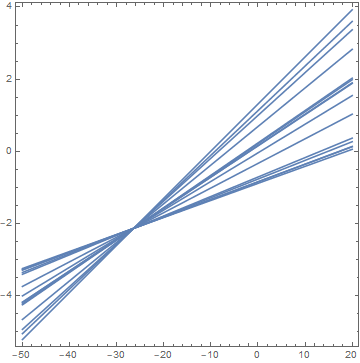
\includegraphics[width=\linewidth]{images/LPrime_PC2_F_Constraint.png}
	\caption[Epipolarlinien in $C'$ aus singulärer Fundamentalmatrix ]{Die Abbildung zeigt, dass die Epipolarlinien auf der Aufnahme von $C'$, nach dem Erzwingen der singularität in der normierten $\hat{F}$, alle durch den Epipol $e'$ verlaufen}
	\label{fig:EpipoleWithF2}
	\endminipage\hfill
	%	\caption{Die mit dem \textit{SURF}-Algorithmus gefundenen Punkte sind mit den gelben Ziffern im Bild gekennzeichnet}
\end{figure}

\begin{figure}[!htb]
	\minipage{0.48\textwidth}
	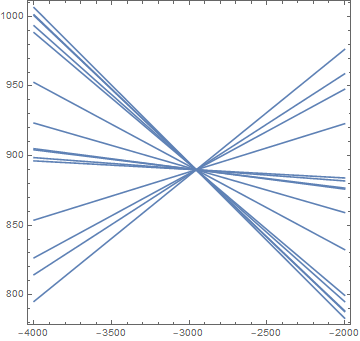
\includegraphics[width=\linewidth]{images/L_PC1_F_Constraint_denormalized.png}
	\caption[Epipolarlinien in $C$ aus singulärer denormalisierter Fundamentalmatrix]{Die Abbildung zeigt die Epipolarlinien in $C$ nachdem die Fundamentalmatrix $\bar{F}$ mit $F = T'\bar{F}T$ denormalisiert wurde}
	\label{fig:EpipoleWithF1Denorm}
	\endminipage\hfill
	\minipage{0.48\textwidth}
	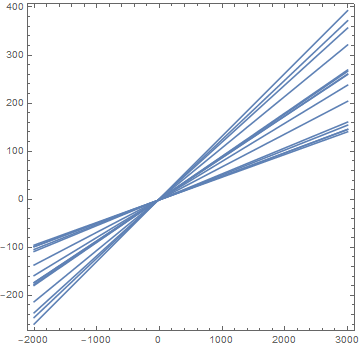
\includegraphics[width=\linewidth]{images/LPrime_PC2_F_Constraint_denormalized.png}
	\caption[Epipolarlinien in $C$ aus singulärer denormalisierter Fundamentalmatrix]{Die Abbildung zeigt die Epipolarlinien in $C'$ nachdem die Fundamentalmatrix $\bar{F}$ mit $F = T'\bar{F}T$ denormalisiert wurde}
	\label{fig:EpipoleWithF2Denorm}
	\endminipage\hfill
	%	\caption{Die mit dem \textit{SURF}-Algorithmus gefundenen Punkte sind mit den gelben Ziffern im Bild gekennzeichnet}
\end{figure}

\pagebreak

\subsection{Singulärwerte der essentiellen Matrix}

Die essentielle Matrix wird im entwickelten Algorithmus aus der Fundamentalmatrix $F$ bestimmt. Da zuvor die singularität von $F$ erzwungen wurde, ist die essentielle Matrix ebenfalls eine Matrix von Rang 2\cite{HZ}. Im synthetischen Beispiel wurde gezeigt, dass für die Bestimmung der extrinsischen Kameraparameter für $E$ gelten muss, dass für ihre Singulärwerte $\Sigma = \text{diag}(1,1,0)$ sind. \\

Die Ungenauigkeit der Punktekorrespondenzen, kann auf $E$ die Auswirkung haben, dass ihre Singulärwerte die Form $\Sigma = \text{diag}(a,b,c)$ mit $a \geq b \geq c$ annehmen. Eine Matrix gilt nur dann als essentielle Matrix, wenn zwei ihrer Singulärwerte gleich sind $(a = b)$ und für den dritten gilt $(c=0)$. Um diese Bedingung zu erzwingen, wird diejenige essentielle Matirix $\hat{E}$ gesucht, welche sich laut der Frobenius Norm am nächsten an der ursprünglichen $E$ befindet\cite{HZ,Ferid}. Diese Matrix lässt sich aus $E = U \Sigma V^T$ bestimmen, indem eine neue essentielle Matrix $\hat{E} = U \hat{\Sigma}V^T$ mit $\hat{\Sigma} = \text{diag}(\frac{a+b}{2},\frac{a+b}{2},0)$\cite{HZ} gebildet wird.\\

Nach erzwingen der singulären Bedingung $\hat{\Sigma} = \text{diag}(\frac{a+b}{2},\frac{a+b}{2},0)$, ist $E$ wieder eine gültige essentielle Matrix und der Algorithmus kann mit der Bestimmung der extrinsischen Kameraparameter, wie in Kapitel \ref{sec:minimal} gezeigt, fortfahren.\\

Das Erzwingen der singulären Bedingungen für $F$ und $E$ sind Näherungsverfahren, in welchen die Auswirkungen der Fehlerhaften Punktekorrespondenzen minimiert werden. Nur wenn $F$ und $E$ ihre singulären Bedingungen erfüllen, können die extrinsischen Kameraparameter bestimmt und die Szene rekonstruiert werden\cite{HZ}.

\section{Szenenrekonstruktion mit Sampson-Approximation}
\label{sec:sampson}

Aufgrund der Ungenauigkeit der korrespondierenden Punkte ist es nicht möglich die 3D-Objektpunkte durch einfache Rückprojektion der Bildpunkte zu rekonstruieren. Liegt der zu $m_\sigma$ korrespondierende Bildpunkt $m'_{\sigma'}$ nicht ganz genau auf der zu $m_\sigma$ korrespondierenden Epipolarlinie, so ist die in Kapitel \ref{sec:HFE} aufgestellte epipolare Bedingung aus Gleichung \ref{eq:Ep6} nicht mehr erfüllt. Durch einsetzten der detektierten korrespondierenden Punkte $m_\sigma$ und $m'_{\sigma'}$ in die Gleichung 

\begin{gather}
	m'^T_{\sigma'}Fm_\sigma = 0
\end{gather}

kommt ein Wert $\neq 0$ heraus. Je weiter der Wert von Null abweicht, desto ungenauer ist die Korrespondenz beider Bildpunkte. Dies führt dazu, dass sich bei der Rückprojektion die Linien der Bildpunkte $m_\sigma$ und $m'_{\sigma'}$ nicht im Raum treffen, sondern windschief zueinander liegen. Die Abbildungen \ref{fig:ProblemTraingulation} und \ref{fig:lFm} veranschaulichen die Konsequenz von ungenauen Punktekorrespondenzen.
%
%ist es bei den Fehlerhaften Bildkooridinaten nicht möglich die 3D-Szenenpunkte durch eine einfache Rückprojektion der der Bildpunkte zu einem Punkt im 3D-Raum zu erhalten. 
%
%sagen dass der epipolarconstraint nicht genau erfüllt wird
%
%Grund nennen und an bilder zeigen 
%Im letzten Schritt des Arbeitsprozesses, wird nun noch die Szenen mit Hilfe eines Triangulationsverfahrens rekonstruiert. Wie bereits im Kapitel \nameref{sec:minimal} erwähnt wurde, ist es bei den Fehlerhaften Bildkooridinaten nicht möglich die 3D-Szenenpunkte durch eine einfache Rückprojektion der der Bildpunkte zu einem Punkt im 3D-Raum zu erhalten. 
%
%liegt nur einer der beiden Bildpunkte $m$ oder $m'$ nicht hundert prozentig auf der jeweilgen korrespondierenden Epipolarlinie, so liegen die rückprojizierten Strahlen windschief im Raum. Das liegt daran, dass die Bildpunkte $m$ und $m'$ nicht den \textit{Epipolar-Constraint} $m'^T F m = 0$ erfüllen. Sprich die Gleichungen $m = PM$ und $m' = P'M$ können nicht erfüllt werden, da es kein $M$ gibt, dass für beide Gleichungen mit den momentanen $m$ und $m'$ gibt. Abbildung 6.11 veranschaulicht die Rückprojektion der Kamerazentren durch zwei Fehlerhafte Bildpunkte. 

\begin{figure}[!htb]
	\minipage{0.48\textwidth}
	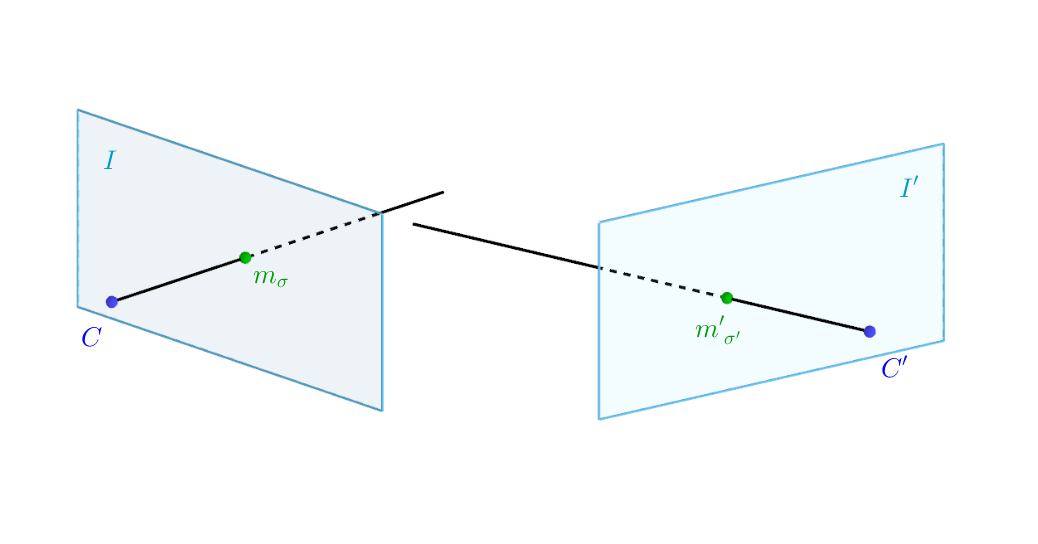
\includegraphics[width=\linewidth]{images/problemTriangulation_beschriftet.png}
	\caption[Windschiefe Geraden]{a) Windschiefe Geraden}
	\label{fig:ProblemTraingulation}
	\endminipage\hfill
	\minipage{0.5\textwidth}
	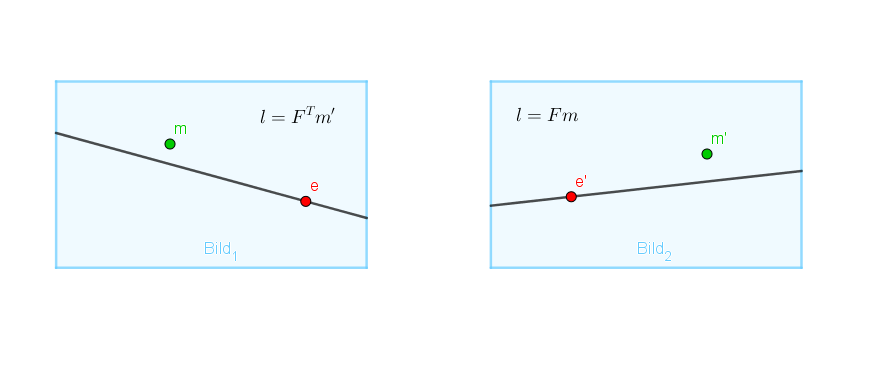
\includegraphics[width=\linewidth]{images/SampsAppx.png}
	\caption[Epipolare Bedingung wird nicht erfüllt]{b) Epipolare Bedingungen werden nicht erfüllt}
	\label{fig:lFm}
	\endminipage\hfill
	\caption[Problemstellung für die Triangulation im reellen Beispiel]{ a) Die rückprojizierten Strahlen der ungenauen korrespondierenden Punkte $m_\sigma$ und $m'_{\sigma'}$ sind Windschief zueinander und treffen sich nicht in einem Punkt $M_{\delta,0}$ im Raum. b) Die korrespondierenden Bildpunkte $m_\sigma$ und $m'_{\sigma'}$ erfüllen nicht die Epipolaren Bedingungen. Die Epipolarlinie $l' = Fm$ ist die korrespondierende Epipolarlinie zu $m_\sigma$ und $l = F^Tm'$ ist die korrespondierende Epipolarlinie zu $m'_{\sigma}$. Da weder $m_\sigma$ noch $m'_{\sigma'}$ auf der Epipolarlinie zum jeweils korrespondierenden Punkt liegen, kommt es zu keinem Schnittpunkt der rückprojizierten Strahlen}
\end{figure}

Um trotz der ungenauen korrespondierenden Punkte eine Triangulation zu ermöglichen, wird ein Verfahren voran geschaltet, welches zwei Punkte $\hat{m}_\sigma$ und $\hat{m}'_{\sigma'}$ sucht, die möglichst nah an den ursprünglichen Punkten $m_\sigma$ und $m'_{\sigma'}$ liegen und gleichzeitig die epipolare Bedingung $\hat{m}'^T_{\sigma'}F\hat{m}_\sigma = 0$ erfüllen. $\hat{m}_\sigma$ und $\hat{m}'_{\sigma'}$ sollen durch Minimierung einer Funktion $C$ bestimmt werden, welche die Distanz  $d$ zwischen $m_\sigma$ und $\hat{m}_\sigma$ und $m'_{\sigma'}$ und $\hat{m}'_{\sigma'}$ minimiert. Für die Minimierung wird das Verfahren der Sampson-Approximation gewählt\cite{HZ}. 

%Voraussetzung für die auf die Minimierung folgende Triangulierung ist, dass die Projektionsmatrizen $P$ und $P'$, sowie die Fundamentalmatrix $F$ bekannt sein müssen\cite{HZ}.

\begin{gather}
	C(m,m') = d(m,\hat{m})^2 + d(m',\hat{m'})^2
\end{gather}

%Jedes Punktepaar, welches den \textit{Epipolar-Constraint} erfüllt, liegt auf einem paar korrespondierender Epipolarlinien. 

Die optimalen Punkte $\hat{m}$ und $\hat{m}'$ liegen auf den korrespondierenden Epipolarlinien $\hat{l}$ und $\hat{l}'$ am Fuße des Lots, welches von den ursprünglich projizierten Punkten $m$ und $m'$ auf die Epipolarlinien $\hat{l}$ und $\hat{l'}$ gefällt wird\cite{HZ}. 


\begin{figure}[!htb]
	\centering
	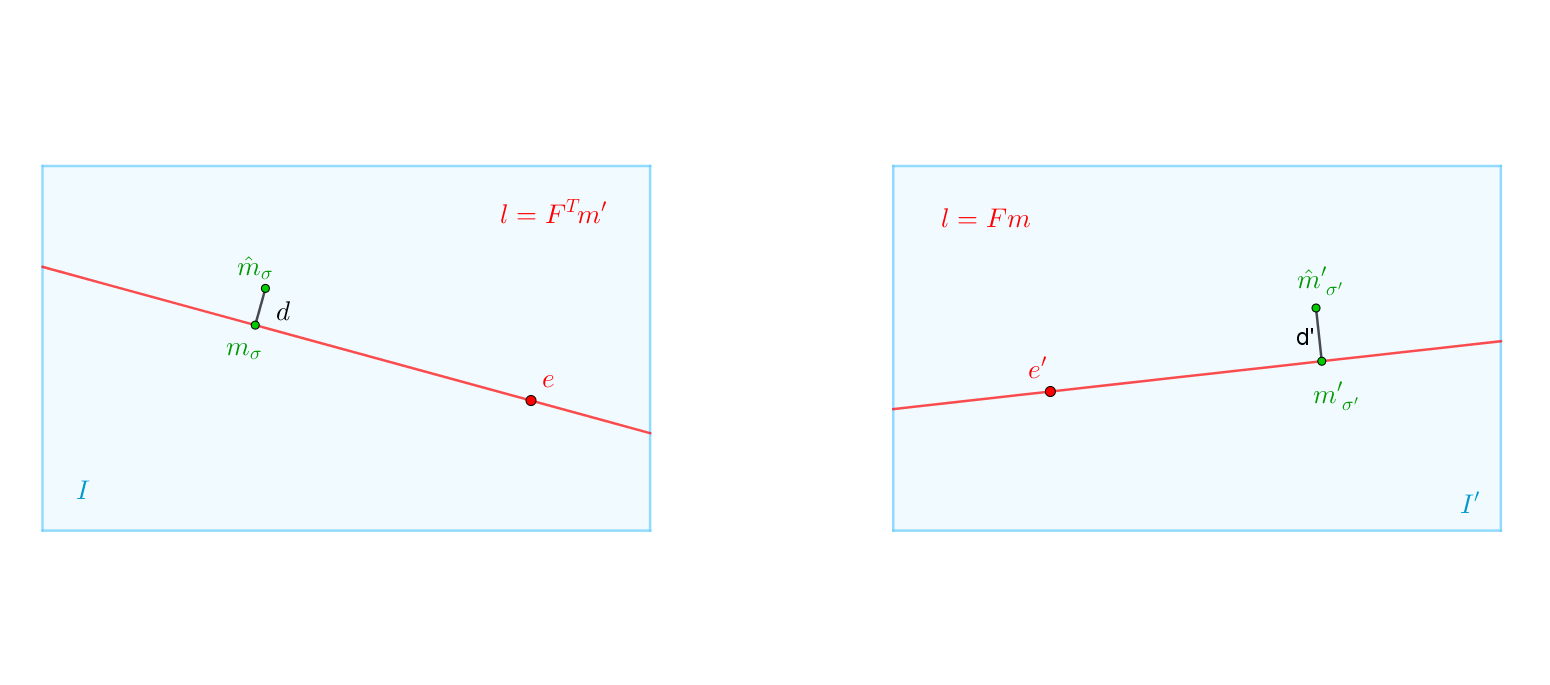
\includegraphics[width=.8\linewidth]{images/SampsAppxNewPoints.png}
	\caption[Sampson Approximation aufstellen der Kostenfunktion]{Die Abbildung zeigt die zwei korrespondierenden Epipolarlinien $\hat{l}$ und $\hat{l'}$ mit den gesuchten Punkten $\hat{m_\sigma}$ und $\hat{m'_{\sigma'}}$}
\end{figure}

%\begin{minipage}{\linewidth}
%	\centering
%	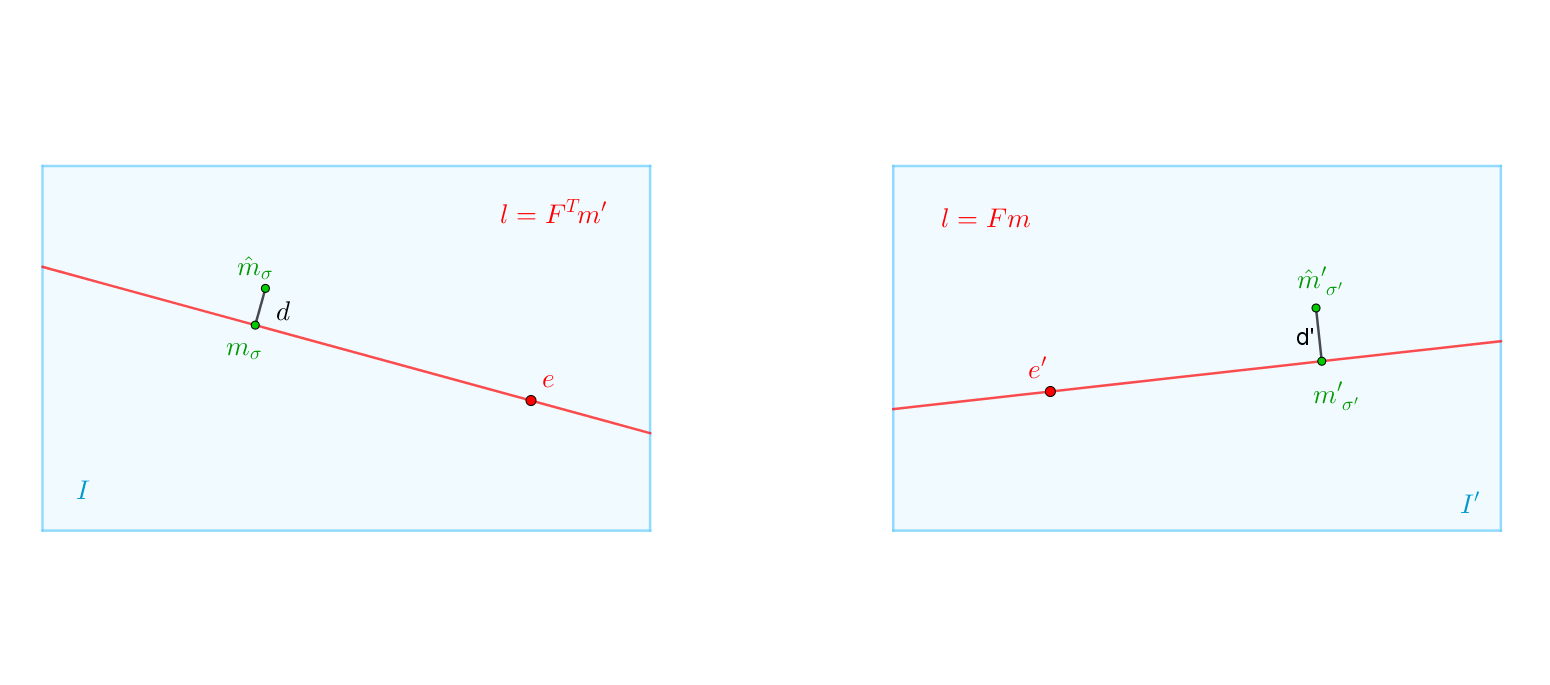
\includegraphics[width=.8\linewidth]{images/SampsAppxNewPoints.png}
%	\captionof{figure}{Die Abbildung zeigt die zwei korrespondierenden Epipolarlinien $\hat{l}$ und $\hat{l'}$ mit den gesuchten Punkten $\hat{m_\sigma}$ und $\hat{m'_{\sigma'}}$}
%\end{minipage}\\\\

Jedes andere Punktepaar auf $\hat{l}$ und $\hat{l}'$ würde die epipolare Bedingung erfüllen, jedoch minimieren nur $m_{\sigma\bot}$ und $m'_{\sigma' \bot}$ die quadratischen Distanzen $d(m_\sigma,\hat{m}_\sigma)^2$ und $ d(m'_{\sigma'},\hat{m}'_{\sigma'})^2$ in der Funktion $C$. Gesucht wird also der geringste Abstand von $m_\sigma$ zu $\hat{l}$ und $m'_{\sigma'}$ zu $\hat{l}'$. Die Funktion $C$ kann dem entsprechend umformuliert werden in 

\begin{gather}
	C(m,m') = d(\hat{m}_\sigma,\hat{l})^2 + d(\hat{m}'_{\sigma'},\hat{l}')^2
\end{gather}
.

Aus allen möglichen Epipolarlinien, welche $\hat{l}$ und $\hat{l}'$ annehmen können, entspricht immer der senkrechte Abstand von $m_\sigma$ und $m'_{\sigma'}$ zur jeweiligen Epipolarlinie der minimalen Distanz. Es soll jedoch genau das Epipolalinienpaar gewählt werden, welches die Funktion $C$ minimal werden lässt\cite{HZ}.\\

Im ersten Schritt werden die Epipolarlinien parametrisiert, so dass eine Linie als $\hat{l}(t)$ geschrieben werden kann. Durch die Parametrisierung der Epipolarlinien, kann die Funktion $C$ als eine Funktion von $t$ umformuliert werden.


\begin{gather}
	C(m_\sigma,m'_{\sigma'}) = d(m_\sigma,\hat{l}(t))^2 + d(m'_{\sigma'},\hat{l}'(t))^2
\end{gather}


%Danach wird die Fundamentalmatrix $F$ dazu benutzt, die entsprechend korrespondierende Epiploarlinie $l'$ zu berechnen. Die Kostenfunktion $C$ kann somit als eine Funktion von $t$ definiert werden. Schlussendlich muss ein Wert für $t$ gefunden werden, welcher $C$ minimal werden lässt. 
%
%\begin{gather}
%	C(m,m') = d(m,\hat{m})^2 + d(m',\hat{m'})^2\\
%	\leadsto 
%	C(m,m') = d(m,l(t))^2 + d(m',l'(t))^2
%\end{gather}\\
%
%Um zu verhindern dass Bildpunkte, die mit dem Epipol des anderen Bildes korrespondieren 
%Korrespondiert ein Bildpunkt dem Epipol eines anderen Bildes, 
%Bei Bildpunkten, welche mit dem Epipol des anderen Bildes korrespondieren, würde sich der rückprojizierte Objektpunkt $M_\delta$ auf der Basislinie der zwei Projektionszentren befinden. Eine Rekonstruktion des Punktes wäre nicht möglich\cite{HZ}.
Um die Minimierung zu vereinfachen, werden zu Beginn die Bildpunkte $m_\sigma$ und $m'_{\sigma'} $ mit jeweils einer Matrix $T$ und $T'$ in den Ursprung $(0,0,1)^T$ verschoben. 


%Es kann passieren , dass ein Bildpunkt korrespondierend zum jeweiligen Epipol des anderen Bildes ist, der Rückprojizierte Punkt im 3D-Raum würde sich dann auf der Basislinie der zwei Projektionszentren befinden und es ist somit nicht möglich ihn zu rekonstruieren. Um solche Fälle zu vermeiden, wird eine Transformation der Punkte $m$ und $m'$ in den Ursprung $(0,0,1)^T$ zu verschieben.

\begin{gather}
	T = \begin{bmatrix}
	1&0&-m_{\sigma x}\\
	0&1&-m_{\sigma y}\\
	0&0&1
	\end{bmatrix} \leadsto \bar{m_\sigma} = T\cdot m_\sigma\\
	T' = \begin{bmatrix}
	1&0&-m'_{\sigma'x}\\
	0&1&-m'_{\sigma'y}\\
	0&0&1
	\end{bmatrix} \leadsto 	\bar{m}'_{\sigma'} = T' \cdot m'_{\sigma'}
\end{gather} \\

Die Fundamentalmatrix $F$ wird ebenfalls mit $T$ und $T'$ transformiert, sodass sie an die verschobenen Punkte $\bar{m}_{\sigma}$ und $\bar{m}'_{\sigma'}$ angepasst ist.
%
%Die Fundamentalmatrix $F$ wird dann wieder an die neu translatierten Punkte $\bar{m}$ und $\bar{m}'$ angepasst.

\begin{gather}
	\bar{F}= T'^{-T}FT^{-1}
\end{gather}

%Als nächstes wird $F$ mit $T$ und $T$ so Transformiert, dass den \textit{Singularity-Constraint} zwischen 
Der rechte und linke Kern von $\bar{F}$ ergeben die Epipole $\bar{e}$ und $\bar{e}'$. Angenommen $f$ und $f'$ seinen genau Null, so liegen die Epipole $e = (1,0,f)^T$ und $e' = (1,0,f')^T$ im unendlichen. Ist dies der Fall so hat $\bar{F}$ für welche dann gilt, dass $\bar{F}(1,0,f)^T = (1,0,f')\bar{F}=0$ eine spezielle Form\cite{HZ}.

%Die entstehenden Epipole besitzen die Form $\hat{e}=(1,0,f)^T$ und $\hat{e'}=(1,0,f')^T$, wobei $f$ und $f'$ nahezu null sein wird. Sollten die $x$ und $y$ Werte der Epipole abweichen, so werden diese so skaliert, dass $\hat{e}^2_x + \hat{e}^2_y = 1$ ergeben, selbiges gilt auch für $\hat{e}'$.


%Des Weiteren sollen die Epipole auf die x-Achse an die Punkte $\hat{e}=(1,0,f)^T$ und $\hat{e'}=(1,0,f')^T$, wobei $f$ und $f'$ nahezu null sein werden. 

%Sind $f = 0$ und $f' = 0$, so liefen die Epipole im unendlichen. Die Epipole lassen sich durch den rechten und linken Kern der neuen $\bar{F}$ berechnen. 



\begin{gather}
	\bar{F} = \begin{pmatrix}
	ff'd&-f'c&-f'd\\
	-fb&a&b\\
	-fd&c&d\label{eq:FSampson}
	\end{pmatrix}\\
	\begin{pmatrix}
	ff'd&-f'c&-f'd\\
	-fb&a&b\\
	-fd&c&d
	\end{pmatrix} \cdot \begin{pmatrix}
	1\\0\\f
	\end{pmatrix} = 
	\begin{pmatrix}
	ff'd + (-ff'd)\\
	-fb + fb\\
	-fd +fd
	\end{pmatrix}
	= 
	\begin{pmatrix}
	0\\0\\0
	\end{pmatrix}\\
	\begin{pmatrix}
	1&0&f'
	\end{pmatrix} \cdot
	\begin{pmatrix}
	ff'd&-f'c&-f'd\\
	-fb&a&b\\
	-fd&c&d
	\end{pmatrix} =
	\begin{pmatrix}
	ff'd + (-ff'd)\\
	-f'c + f'c\\
	-f'd + f'd
	\end{pmatrix} = 
		\begin{pmatrix}
	0&0&0
	\end{pmatrix}
\end{gather}

Im Realfall sind die Werte der Epipole $e$ und $e'$ nicht genau $e = (1,0,f)^T$ und $e' = (1,0,f')^T$, sondern weichen in ihren Richtungen leicht ab. Des Weiteren sind die Epipole auch noch nicht normiert. Es folgt zunächst die Normierung der Epipole, sodass $e^2_1 + e^2_2 = 1$ und $e'^2_1 + e'^2_2 = 1$ gilt. Danach werden $e$ und $e'$ mit zwei Rotationsmatrizen $R$ und $R'$ auf $Re = (1,0,e_3) = (1,0,f)$ und $R'e' = (1,0,e'_3)=(1,0,f')$ rotiert.

\begin{gather}
	R = \begin{bmatrix}
		e_1&e_2&0\\
		-e_2&e_1&0\\
		0&0&1
	\end{bmatrix}\\
	R' = \begin{bmatrix}
	e'_1&e'_2&0\\
	-e'_2&e'_1&0\\
	0&0&1
\end{bmatrix}
\end{gather}\\

$\bar{F}$ wird dann mit $\bar{F}_{Rot} = R'FR^T$ ersetzt. Die Einträge in $\bar{F}_{Rot}$ haben nun die Form wie in Gleichung \ref{eq:FSampson}, mit $f = e_3, \, f' = e'_3, \, a = \bar{F}_{Rot,22}, \, b = \bar{F}_{Rot,23}, \, c = \bar{F}_{Rot,32}$ und $d = \bar{F}_{Rot,33}$.

\begin{gather}
	\bar{F}_{Rot} = 
\begin{pmatrix}
	e_3e'_3 \bar{F}_{Rot,33}&-e'_3 \bar{F}_{Rot,32}&-e'_3\bar{F}_{Rot,33}\\
	-e_3 \bar{F}_{Rot,23} & \bar{F}_{Rot,22} &\bar{F}_{Rot,23}\\
	-e_3 \bar{F}_{Rot,33}& \bar{F}_{Rot,32} &\bar{F}_{Rot,33} \label{eq:SampsonFRot}
\end{pmatrix}
\end{gather}
Verläuft eine Epipolarlinie durch einen Punkt $(0,t,1)^T$ und dem Epipol $e = (1,0,f)^T$, wird diese Epipolarlinie mit $l(t)$ bezeichnet. Das Kreuzprodukt dieser beiden Punkte beschreibt die Epipolarlinie $l(t)$\cite{HZ}. %\pagebreak

\begin{gather}
\hat{l}(t)=
	\begin{pmatrix}
	0\\t\\1
	\end{pmatrix} \times
	\begin{pmatrix}
	1\\0\\f
	\end{pmatrix} = 
	\begin{pmatrix}
	tf\\1\\-t
	\end{pmatrix}
\end{gather}

Die quadratische Distanz dieser Linie zum Ursprung wird dann bezeichnet mit:


\begin{gather}
	d(\bar{m_\sigma},\hat{l}(t))^2 = \frac{t^2}{1+(tf)^2} \label{eq:quadraticDistance}
\end{gather}

Nach \textit{Hartley \& Zisserman} \cite{HZ} werden Linien durch Vektoren der Form $\vec{v} = \begin{pmatrix}
A\\B\\C
\end{pmatrix}$ dargestellt. Übersetzt in eine Koordinatengleichung ergibt sich

\begin{gather}
	Ax+By+C = 0
\end{gather}.

Die Gleichung \ref{eq:quadraticDistance} wird anhand der Koordinatengleichung hergeleitet. Für die Herleitung wird die Koordinatenform der Geraden zunächst in Normalform umgeschrieben

%\begin{gather}
%	Ax+By-C = 0
%\end{gather}
%
%Die Selbe Gerade in Normalform ausgedrückt lautet:

\begin{gather}
\vec{n}\cdot (\vec{x} - \vec{p}) = 0\\
	\begin{pmatrix}
	A\\B
	\end{pmatrix}
	\cdot
	(\vec{x} - \begin{pmatrix}
		0\\ \frac{C}{B}
	\end{pmatrix}) = 0\label{eq:GeradengleichungSampson}
\end{gather} .

Der Abstand $\parallel \vec{v} \parallel$ eines Punktes zur Geraden \ref{eq:GeradengleichungSampson} kann folgendermaßen berechnet werden.

\begin{gather}
	\vec{v} = \frac{\vec{p} \cdot \vec{n}}{\vec{n} \cdot \vec{n}} \cdot \vec{n}
	\leadsto \frac{-C}{A^2+B^2} \cdot \begin{pmatrix}
	A\\B
	\end{pmatrix}\\
	||\vec{v}|| = \frac{|\vec{p} \cdot \vec{n}|}{||\vec{n}||^2} \cdot ||\vec{n}|| \leadsto ||\vec{v}|| = \frac{|\vec{p} \cdot \vec{n}|}{||\vec{n}||}\\
	\Rightarrow |C| = |\vec{p} \cdot \vec{n}| \\
	\Rightarrow |\sqrt{A^2+B^2}| = ||\vec{n}||\\
	||\vec{v}|| = \frac{|C|}{\sqrt{A^2+B^2}}
\end{gather}

Werden nun $A,B$ und $C$ mit den Werten der Geraden $(tf,1,-t)^T$ ersetzt, kann Gleichung \ref{eq:quadraticDistance} rekonstruiert werden.

\begin{gather}
	A = tf, \; B= 1, \; C = -t, \; \vec{v} = d\\
	d^2 = \frac{t^2}{\sqrt{((tf)^2+1^2)^2}} = \frac{t^2}{(tf)^2+ 1^2} =  \frac{t^2}{1 + (tf)^2}
\end{gather}\\

Um die zu $\hat{l}(t)$ korresponiderende Epipolarlinie $\hat{l}'(t)$ zu bestimmen, wird der Beispielpunkt $(0,t,1)^T$ und die Fundamentalmatrix $\bar{F}_{Rot}$ multipliziert. Für die Übersichtlichkeit der Matrix  $\bar{F}_{Rot}$, wird die Symbolschreibweise aus Gleichung \ref{eq:FSampson} genutzt. Für die Einträge gelten die Definitionen aus Gleichung \ref{eq:SampsonFRot}.

\begin{gather}
	l'(t) = \bar{F}_{Rot}(0,t,1)^T = (-f'(ct+d),at+b,ct+d)^T.
\end{gather}

Für die quadratische Distanz $d(\bar{m}'_{\sigma'},l'(t))^2$ ergibt sich dann:

\begin{gather}
	d(\bar{m}'_{\sigma'},l'(t))^2 = \frac{(ct + d)^2}{(at+b)^2+f'^2(ct+d)^2}
\end{gather} \\

Die Funktion $C$ kann jetzt in eine Funktion von $s(t)$ umformuliert werden.

\begin{gather}
%	C(m,m') = d(m,\hat{m})^2 + d(m',\hat{m'})^2 \\
%	\leadsto 	C(m,m') = d(m,l(t))^2 + d(m',l'(t))^2\\
	s(t) = \frac{t^2}{1+(tf)^2} + \frac{(ct + d)^2}{(at+b)^2+f'^2(ct+d)^2}
\end{gather}

Ein Minimum für $s(t)$ kann beispielsweise durch Bestimmung der Minima und Maxima mit $s'(t) = 0$ gefunden werden. 

\begin{gather}
	s'(t) = \frac{2t}{(1+f^2t^2)^2} - \frac{2(ad-bc)(at+b)(ct+t)}{((at+b)^2+f'^2(ct+d)^2)^2}
\end{gather}

Werden die beiden Terme in $s'(t)$ auf einen gemeinsamen Nenner gebracht und der Zähler dann gleich Null gesetzt, ergibt sich der folgende Ausdruck $g(t)$\cite{HZ}

\begin{gather}
	g(t) = t((at+b)^2+f'^2(ct+d)^2)^2-(ad-bc)(1+f^2t^2)^2(at+b)(ct+d)
\end{gather}.

Funktion $g(t)$ ist ein Polynom vom Grad 6. Das Minimum für $s(t)$ ergibt sich aus einer der sechs möglichen Lösungen für $t$ aus $g(t)$. Für die Bestimmung des Minimums werden nur die reellen Lösungen für $t$ in Betracht gezogen. Die reellen Lösungen für $t$ aus $g(t)$, werden dann wieder in $s(t)$ eingesetzt. Das $t$, welches durch einsetzten in $s(t)$ den kleinsten Wert ergibt, ist das gesuchte Minimum $t_{min}$. \\

Mit $t_{min}$ können die Epipolarlinien $\hat{l}(t_{min})=(t_{min}f,1,-t)$ und $\hat{l}'(t_{min}) = \bar{F}_{Rot}(0,t_{min},1)^T$ berechnet werden. Danach werden die zwei neuen Punkte $\hat{m}_{\sigma Rot}$ und $\hat{m}'_{\sigma' Rot}$ auf den Epipolarlinien $\hat{l}(t_{min})$ und $\hat{l}'(t_{min})$ bestimmt. $\hat{m}_{\sigma Rot}$ und $\hat{m}'_{\sigma' Rot}$ sind die Punkte auf der Epipolarlinie welche dem Ursprung am nächsten sind. Zur Erinnerung die Bildpunkte $m_\sigma$ und $m'_{\sigma'}$ wurden zu Beginn in den Ursprung verschoben. Der Punkt, welcher vom Ursprung aus am nächsten auf einer Linien $(\lambda, \mu,\upsilon)$ liegt, kann mit $(-\lambda \cdot \upsilon, -\mu \cdot \upsilon, \lambda^2+ \mu^2)$ berechnet werden\cite{HZ}. Somi gilt

\begin{gather}
	\hat{l} = (tf, 1, -t)\\
	\hat{m}_{\sigma Rot} = (-(tf) \cdot \upsilon , - 1 \cdot \upsilon, (tf)^2 \cdot 1^2 )\\
\end{gather}.
 
Nachdem zu beiden Linien $\hat{l}$ und $\hat{l}'$ der jeweils nächste Punkte $\hat{m}_{Rot}$ und $\hat{m}'_{Rot}$ vom Ursprung aus gefunden wurden, werden diese nun mit $T$, $T'$, $R$ und $R'$ wieder an ihre Ausgangsposition zurück Transformiert. 

\begin{gather}
	\hat{m} = T^{-1}R^T\hat{m}_{Rot}\\
	\hat{m}' = T'^{-1}R'^T\hat{m}'_{Rot}
\end{gather}

%Vergleicht man die Punkte $m$ und $\hat{m}$ und die Punkte $m'$ und $\hat{m'}$, so kann die minimalen Abweichungen der Punkte voneinander sehen. 


Für diese neu berechneten korrespondierenden Punkte ist die epipolare Bedingung aus Gleichung \ref{eq:Ep6} erfüllt und es ist gewährleistest, dass sich ihre jeweiligen Rückprojektionen in einem Punkt im Raum treffen.\\

Für die Rückprojektion der einzelnen Bildpunkte wurde ein lineares Triangulationsverfahren gewählt\cite{HZ}. Dieses ist für mehrere Punkte rechentechnisch günstiger als das geometrische Verfahren, welches im synthetischen Beispiel in Kapitel \ref{sec:minimal} genutzt wurde.\\

Für die Rückprojektion werden pro korrespondierendem Punktepaar zunächst die Projektionsgleichungen  $\hat{m}_\sigma = P\hat{M}_\delta$ und $\hat{m}'_{\sigma'}  = P'\hat{M}_\delta$ aufgestellt. Diese werden so in eine Koeffizientenmatrix $A$ eingetragen dass gilt $A\cdot x = 0$. Durch die Verwendung des Kreuzproduktes, wird die homogene Komponente eliminiert\cite{HZ}. 

%(HIER WEITER MACHEN)
%Nachdem nun gewährleistet ist, dass sich Rückprojektion der neuen Punkte $\hat{m}_\tau$ und $\hat{m}'_{\tau'}$


%Um nun noch den Punkt $\hat{M}$ im 3D-Raum zu rekonstruieren, kann nun jegliche bekannte Methode für die Triangulierung verwendet werden. Durch die zuvorigen Rechenoperationen ist nun gewährleistet, dass sich die Gerade der Projektionszentren $C$ und $C'$ durch ihre jeweiligen Bildpunkte $\hat{m}$ und $\hat{m}'$ auf jeden Fall im Raum treffen\cite{HZ}. Für Doe Rückprojektion der Punkte $\hat{m}$ und $\hat{m}'$ zu $\hat{M}$ wurde ebefalls sich wieder auf ein Verfahren von \textit{Hartley \& Zisserman} berufen. Es handelt sich um eine lineare Triangulierungsmethode.

\begin{gather}
	\hat{m}_\sigma \times (PM_\delta) = 0\\
	\hat{m}'_{\sigma'} \times (PM_\delta) = 0
\end{gather}

Was ausgeschrieben für $\hat{m}$ und $\hat{m}'$ zu den folgenden drei Gleichungen führt. $\hat{m}_\sigma \times (PM_\delta) = 0$ ergibt ausgeschrieben

\begin{gather}
m_{\sigma\,x}(p^{3T}M_\delta) - (p^{1T}M_\delta)=0\\
m_{\sigma\,y}(p^{3T}M_\delta) - (p^{2T}M_\delta)=0\\
m_{\sigma\,x}(p^{2T}M_\delta) - m_{\sigma\,y}(p^{1T}M_\delta)=0
\end{gather}.

und Für $\hat{m}'_{\sigma'} \times (PM_\delta) = 0$ gelten


\begin{gather}
	m'_{\sigma'\,x}(p^{3T}M_\delta) - (p^{1T}M_\delta)=0\\
	m'_{\sigma'\,y}(p^{3T}M_\delta) - (p^{2T}M_\delta)=0\\
	m'_{\sigma'\,x}(p^{2T}M_\delta) - m'_{\sigma'\,y}(p^{1T}M_\delta)=0
\end{gather}.

$p^{iT}$ bezeichnet hier jeweils die Reihen der Projektionsmatrix $P$ beziehungsweise $P'$. Zwei der drei Gleichungen sind linear unabhängig und werden in die Koeffizietenmatrix $A$ geschrieben 


% Die Matrix $A$ stellt sich, aufgrund der Tatsache, dass die Komponenten der Gleichungen 7.37 bis 7.39 linear zu $\hat{M}$ sind, wie folgt zusammen.

\begin{gather}
A = \begin{bmatrix}
xp^{3T}-p^{1T}\\
yp^{3T}-p^{2T}\\
x'p'^{3T}-p'^{^T}\\
y'p'^{3T}-p'^{2T}
\end{bmatrix}\\
%A = \begin{bmatrix}
%	xp^{3T}-p^{1T}\\
%	yp^{3T}-p^{2T}\\
%	x'p'^{3T}-p'^{^T}\\
%	y'p'^{3T}-p'^{2T}
%\end{bmatrix}
\end{gather}\\

Die zwei Wege eine solche Matrix zu lösen wurden in Kapitel \ref{sec:HFE} vorgestellt. Zum einen kann die inhomogene Methode angewandt werden in welcher die Bestimmung des Kerns das Ergebnis für $M_{\delta,0}$ bietet oder es kann das homogene Verfahren angewandt werden, welches die Methode der Singulärwertzerlegung beinhaltet. \\

Die rekonstruierten Punkte $M_{\delta 0}$ sind wie in Kapitel \ref{sec:minimal} auch nur bis auf einen skalierungsfaktor genau bestimmt. Die Abbildungen \ref{fig:reconstructedSampson3D} und \ref{fig:reconstructedSampson3D} zeigen die aus den Bildern \ref{fig:SurfLinks} und \ref{fig:SurfRechts} rekonstruierten Punkte im Raum. Der rote Punkt steht für die Position von $C$, der grüne für die Position von $C'$. Die blauen Punkte sind die rekonstruierten Punkte, der beiden Bilder \ref{fig:SurfLinks} und \ref{fig:SurfRechts}. Somit wurde gezeigt, dass der Algorithmus, welcher für die synthetische Rekonstruktion entwickelt wurde, mit gewissen Modifizierungen auch für ein reelles Stereobildpaar angewandt werden kann. Durch die Näherungen, sind gewissen Abweichungen von der Originalszene nicht zu vermeiden.

%
% Abbildung 7.15 zeigt die 3D Szene. Der Rote Punkt simbolisiert die Position von $C$ also der Canon 6D und der grüne Punkt symbolisiert die Position von $C'$ also der Canon 60D. Die Blauen Punkte sind die durch den \textit{SURF}-Algorithmus detektierten Punkte der Szene. Abbildung 7.16 zeigt die rekonstruierten Objektpunkte als 2D-Punkte, hierfür wurden ihre Koordinaten einfach durch ihren Tiefenwert geteilt. 
%
% Hier wird die Singulärwertzerlegung an A durchgeführt und derjenige Vektor gesucht werden, welcher mit dem kleinsten Singulärwert korrespondiert\cite{HZ}. Das Ergebnis ist jeweils $\hat{M}$ im 3D-Raum. Da die vorherige $P$ und $P'$ nur bis zu einem Skalierungsfaktor genau bestimmt wurden, muss nachdem die Punkte rekonstruiert wurden noch die skalierung auf ihre ursprüngliche Größe erfolgen. Dies ist am einfachsten, wenn eine Referenzgröße zuvor in der Originalszene gemessen wurde. Die Abbildungen 7.15 und 7.16 zeigen die Rekonstruierte Szene des Beispiels, jedoch noch nicht skaliert auf ihre Ursprungsgrößen. 

\begin{figure}[!htb]
	\minipage{0.48\textwidth}
	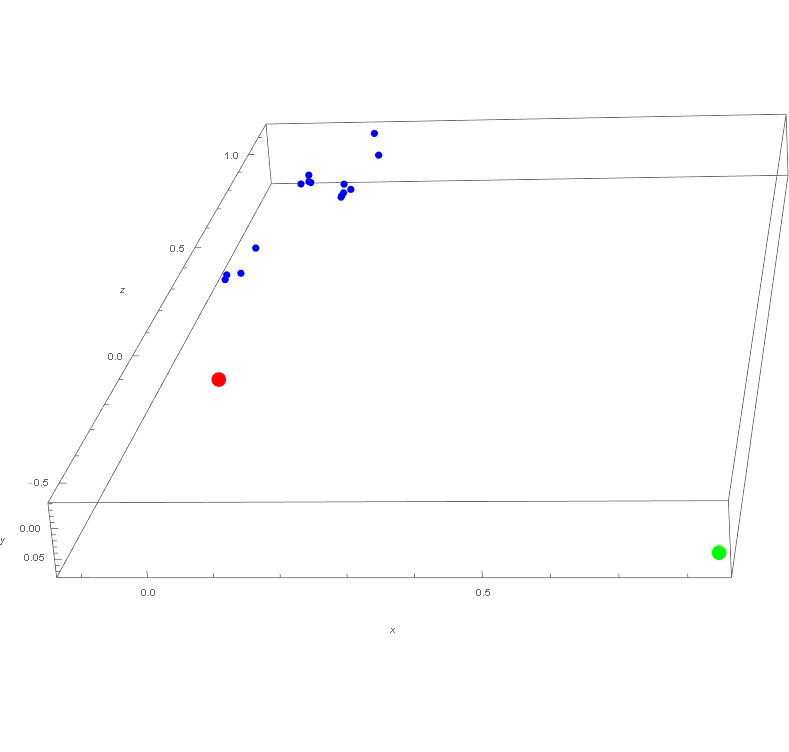
\includegraphics[width=\linewidth]{images/reconstructed_Points_Same_Resolutions.png}
	\caption[Rekonstruierte Szene 3D]{Rekonstruierte Szene, unskaliert in Pixeleinheiten}
	\label{fig:reconstructedSampson3D}
	\endminipage\hfill
	\minipage{0.48\textwidth}
	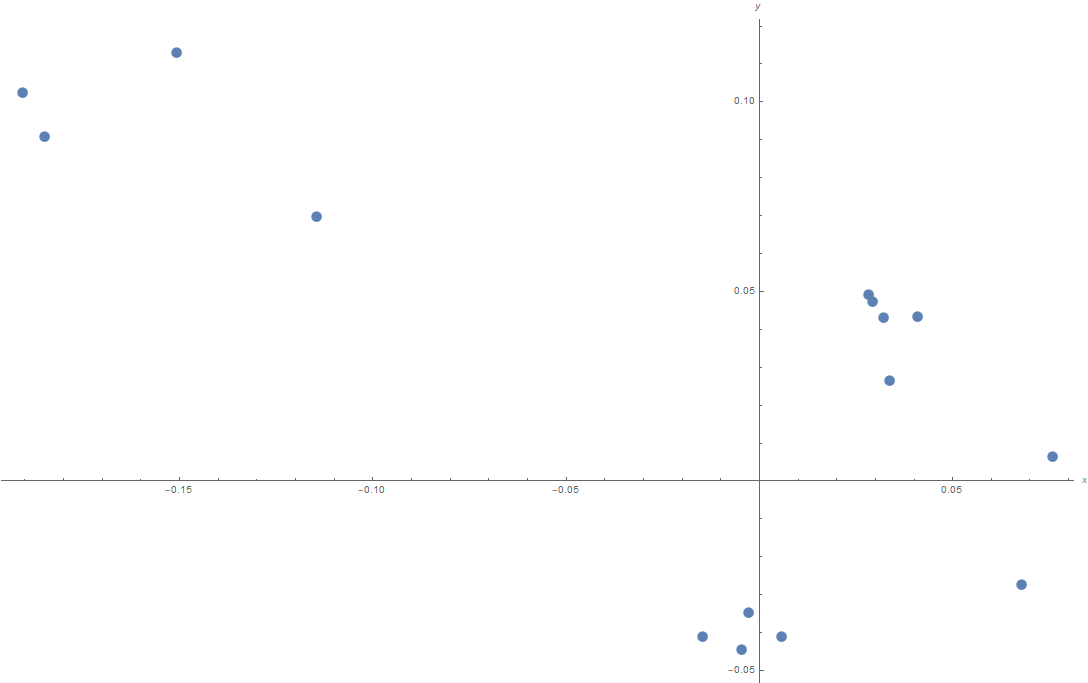
\includegraphics[width=\linewidth]{images/reconstructed_Points_Same_Resolutions2D.png}
	\caption[Rekonstruierte Szene 2D]{Rekonstruierte Szene, unskaliert, in Pixeleinheiten und in einem 2D-Plot angezeigt}
	\label{fig:reconstructedSampson2D}
	\endminipage\hfill
	%	\caption{Die mit dem \textit{SURF}-Algorithmus gefundenen Punkte sind mit den gelben Ziffern im Bild gekennzeichnet}
\end{figure}



%\begin{minipage}{\linewidth}
%	\centering
%	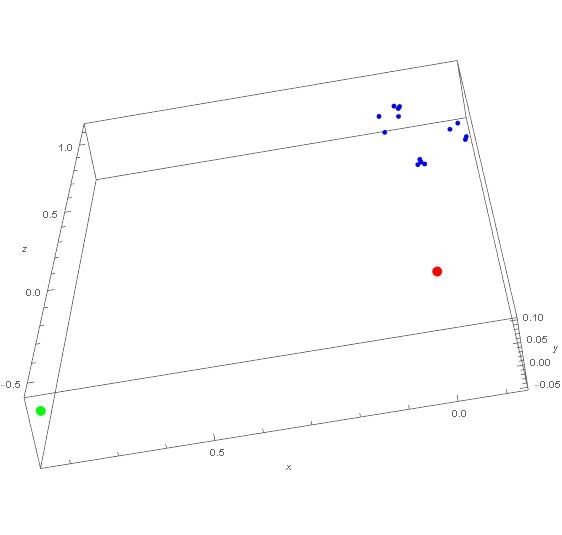
\includegraphics[width=.8\linewidth]{images/result_DetectedmathematicaPointsDifferentResolutions.png}
%	\captionof{figure}{Frafische Darstellung der optimalen Punkte $\hat{m}$ und $\hat{m'}$}
%\end{minipage}\\

%\subsection{andere Ansätze für Triangulationsverfahren}
%Um eine Triangulation zu ermöglichen, muss eine Methode gefunden werden, welche diesen Fehler so weit minimiert, dass es zu einer erfolgreichen Rückprojektion kommt. Die verwendete Methode zur Rekonstruktion der Szene wurde nach der Vorlage von \textit{Hartley \& Zisserman}\cite{HZ} implementiert und wird im folgenden Schritt für Schritt beschrieben.\\
%
%Voraussetzung ist, dass die Projektionsmatrizen $P$ und $P'$, sowie die Fundamentalmatrix $F$ bekannt sein müssen. Sind die Projektionsmatrizen $P$ und $P'$ bis auf eine projektive oder affine Komponenten bekannt, so ist es wünschenswert, wenn die Triangulierung auf einem affinen und projektiv invarianten Verfahren funktioniert\cite{HZ}.\\


%Die hier verwendeten Porjektionsmatrizen sind bis auf eine Skaleninvarianz genau bestimmt, was unter den Fall der affinen invarianz Fällt. Wären die intrinsischen Kameraparameter $K$ und $K'$ nicht bekannt gewesen, gibt es die Möglichkeit die Projektionsmatrizen über die Fundamentalmatrix $F$ mit dem, im Buch von \textit{Hartley \& Zisserman} beschriebenen  \textit{Stratified-Approach} bis auf eine projektive Invarianz genau zu bestimmen\cite{HZ}. 
%
%Die hier verwendete Triangulierung ist nur projektiv invariant, kann aber trotzdem genutzt werden. Die rekonstruierte Szene ist, dann wie im Minimalbeispiel auch, nicht auf ihre Originalmaße skaliert, was aber nach der Triangulierung noch getan werden kann.\\
%
%Die Triangulierung ist deshalb projektiv invariant, weil alle Rechenoperationen, wie die Minimierungen von Distanzen, sich nur auf die 2D-Bildern beziehen und sich nicht in den projektiven 3D-Raum erstreckt\cite{HZ}. \\
%
%Der Grundgedanke der Triangulation ist, dass zwei Punkte $\hat{m}$ und $\hat{m'}$ gefunden werden sollen, die möglichst nah an den ursprünglichen $m$ und $m'$ sind und gleichzeitig den \textit{Epipolar-Constraint} $\hat{x}'^TF\hat{x} = 0$ erfüllen. Dies erfolgt durch die Minimierung einer Kostenfunktion $C$.\\

% In vielen bekannten Computer Vision Applikationen wird für diese Minimierung eine numerische Lösung gewählt, die wohl bekannteste Methode ist der \textit{Levenberg-Marquardt} Algorithmus\cite{HZ}. Jedoch hat sich gezeigt, dass ein nahezu optimales Minimum der geometrischen Kostenfunktion $C$ auch durch eine Annäherung ersten Grades finden lässt. Die Annährung um die es sich handelt ist die sogenannten \textit{Sampson-approximation}


%\subsection{Minimieren der Kostenfunktion durch Sampson-approximation}

%
%Es sollen zwei Punkte $\hat{m}$ und $\hat{m}'$ gefunden werden, welche nahe an den Ursprünglichen $m$ und $m'$ liegen und gleichzeitig den \textit{Epipolar-Constraint} erfüllen. $\hat{m}$ und $\hat{m}'$ sollen durch Minimierung einer Kostenfunktion $C$ ermittelt werden, welche die Distanz  $d$ zwischen $m$ und $\hat{m}$ und $m'$ und $\hat{m'}$ minimiert.
%
%
%\begin{gather}
%	C(m,m') = d(m,\hat{m})^2 + d(m',\hat{m'})^2
%\end{gather}
%
%Die projizierten Punkte $\hat{m}$ und $\hat{m'}$ eines 3D-Objektpunktes $\hat{M}$ liegen auf einem paar korrespondierender Epipolarlinien. 



